%**************************************%
%* Generated from MathBook XML source *%
%*    on 2016-08-13T10:01:07-04:00    *%
%*                                    *%
%*   http://mathbook.pugetsound.edu   *%
%*                                    *%
%**************************************%
\documentclass[10pt,]{book}
%% Load geometry package to allow page margin adjustments
\usepackage{geometry}
\geometry{letterpaper,total={5.0in,9.0in}}
%% Custom Preamble Entries, early (use latex.preamble.early)
%% Inline math delimiters, \(, \), need to be robust
%% 2016-01-31:  latexrelease.sty  supersedes  fixltx2e.sty
%% If  latexrelease.sty  exists, bugfix is in kernel
%% If not, bugfix is in  fixltx2e.sty
%% See:  https://tug.org/TUGboat/tb36-3/tb114ltnews22.pdf
%% and read "Fewer fragile commands" in distribution's  latexchanges.pdf
\IfFileExists{latexrelease.sty}{}{\usepackage{fixltx2e}}
%% Page Layout Adjustments (latex.geometry)
%% This LaTeX file may be compiled with pdflatex, xelatex, or lualatex
%% The following provides engine-specific capabilities
%% Generally, xelatex and lualatex will do better languages other than US English
%% You can pick from the conditional if you will only ever use one engine
\usepackage{ifthen}
\usepackage{ifxetex,ifluatex}
\ifthenelse{\boolean{xetex} \or \boolean{luatex}}{%
%% begin: xelatex and lualatex-specific configuration
%% fontspec package will make Latin Modern (lmodern) the default font
\ifxetex\usepackage{xltxtra}\fi
\usepackage{fontspec}
%% realscripts is the only part of xltxtra relevant to lualatex 
\ifluatex\usepackage{realscripts}\fi
%% 
%% Extensive support for other languages
\usepackage{polyglossia}
\setdefaultlanguage{english}
%% Magyar (Hungarian)
\setotherlanguage{magyar}
%% Spanish
\setotherlanguage{spanish}
%% Vietnamese
\setotherlanguage{vietnamese}
%% end: xelatex and lualatex-specific configuration
}{%
%% begin: pdflatex-specific configuration
%% translate common Unicode to their LaTeX equivalents
%% Also, fontenc with T1 makes CM-Super the default font
%% (\input{ix-utf8enc.dfu} from the "inputenx" package is possible addition (broken?)
\usepackage[T1]{fontenc}
\usepackage[utf8]{inputenc}
%% end: pdflatex-specific configuration
}
%% Monospace font: Inconsolata (zi4)
%% Sponsored by TUG: http://levien.com/type/myfonts/inconsolata.html
%% See package documentation for excellent instructions
%% One caveat, seem to need full file name to locate OTF files
%% Loads the "upquote" package as needed, so we don't have to
%% Upright quotes might come from the  textcomp  package, which we also use
%% We employ the shapely \ell to match Google Font version
%% pdflatex: "varqu" option produces best upright quotes
%% xelatex,lualatex: add StylisticSet 1 for shapely \ell
%% xelatex,lualatex: add StylisticSet 2 for plain zero
%% xelatex,lualatex: we add StylisticSet 3 for upright quotes
%% 
\ifthenelse{\boolean{xetex} \or \boolean{luatex}}{%
%% begin: xelatex and lualatex-specific monospace font
\usepackage{zi4}
\setmonofont[BoldFont=Inconsolatazi4-Bold.otf,StylisticSet={1,3}]{Inconsolatazi4-Regular.otf}
%% end: xelatex and lualatex-specific monospace font
}{%
%% begin: pdflatex-specific monospace font
\usepackage[varqu]{zi4}
%% end: pdflatex-specific monospace font
}
%% Symbols, align environment, bracket-matrix
\usepackage{amsmath}
\usepackage{amssymb}
%% allow more columns to a matrix
%% can make this even bigger by overriding with  latex.preamble.late  processing option
\setcounter{MaxMatrixCols}{30}
%%
%% Color support, xcolor package
%% Always loaded.  Used for:
%% mdframed boxes, add/delete text, author tools
\PassOptionsToPackage{usenames,dvipsnames,svgnames,table}{xcolor}
\usepackage{xcolor}
%%
%% Semantic Macros
%% To preserve meaning in a LaTeX file
%% Only defined here if required in this document
%% Used for inline definitions of terms
\newcommand{\terminology}[1]{\textbf{#1}}
%% Subdivision Numbering, Chapters, Sections, Subsections, etc
%% Subdivision numbers may be turned off at some level ("depth")
%% A section *always* has depth 1, contrary to us counting from the document root
%% The latex default is 3.  If a larger number is present here, then
%% removing this command may make some cross-references ambiguous
%% The precursor variable $numbering-maxlevel is checked for consistency in the common XSL file
\setcounter{secnumdepth}{3}
%% Environments with amsthm package
%% Theorem-like environments in "plain" style, with or without proof
\usepackage{amsthm}
\theoremstyle{plain}
%% Numbering for Theorems, Conjectures, Examples, Figures, etc
%% Controlled by  numbering.theorems.level  processing parameter
%% Always need a theorem environment to set base numbering scheme
%% even if document has no theorems (but has other environments)
\newtheorem{theorem}{Theorem}[section]
%% Only variants actually used in document appear here
%% Style is like a theorem, and for statements without proofs
%% Numbering: all theorem-like numbered consecutively
%% i.e. Corollary 4.3 follows Theorem 4.2
\newtheorem{algorithm}[theorem]{Algorithm}
%% Definition-like environments, normal text
%% Numbering is in sync with theorems, etc
\theoremstyle{definition}
\newtheorem{definition}[theorem]{Definition}
%% Remark-like environments, normal text
%% Numbering is in sync with theorems, etc
\theoremstyle{definition}
\newtheorem{note}[theorem]{Note}
%% Example-like environments, normal text
%% Numbering is in sync with theorems, etc
\theoremstyle{definition}
\newtheorem{example}[theorem]{Example}
%% Miscellaneous environments, normal text
%% Numbering for inline exercises and lists is in sync with theorems, etc
\theoremstyle{definition}
\newtheorem{exercise}[theorem]{Exercise}
%% Localize LaTeX supplied names (possibly none)
\renewcommand*{\chaptername}{Chapter}
%% Figures, Tables, Listings, Floats
%% The [H]ere option of the float package fixes floats in-place,
%% in deference to web usage, where floats are totally irrelevant
%% We re/define the figure, table and listing environments, if used
%%   1) New mbxfigure and/or mbxtable environments are defined with float package
%%   2) Standard LaTeX environments redefined to use new environments
%%   3) Standard LaTeX environments redefined to step theorem counter
%%   4) Counter for new environments is set to the theorem counter before caption
%% You can remove all this figure/table setup, to restore standard LaTeX behavior
%% HOWEVER, numbering of figures/tables AND theorems/examples/remarks, etc
%% WILL ALL de-synchronize with the numbering in the HTML version
%% You can remove the [H] argument of the \newfloat command, to allow flotation and 
%% preserve numbering, BUT the numbering may then appear "out-of-order"
\usepackage{float}
\usepackage[bf]{caption} % http://tex.stackexchange.com/questions/95631/defining-a-new-type-of-floating-environment 
\usepackage{newfloat}
% Figure environment setup so that it no longer floats
\SetupFloatingEnvironment{figure}{fileext=lof,placement={H},within=section,name=Figure}
% figures have the same number as theorems: http://tex.stackexchange.com/questions/16195/how-to-make-equations-figures-and-theorems-use-the-same-numbering-scheme 
\makeatletter
\let\c@figure\c@theorem
\makeatother
%% Raster graphics inclusion, wrapped figures in paragraphs
%% \resizebox sometimes used for images in side-by-side layout
\usepackage{graphicx}
%%
%% Program listing support, for inline code, Sage code
\usepackage{listings}
%% We define the listings font style to be the default "ttfamily"
%% To fix hyphens/dashes rendered in PDF as fancy minus signs by listing
%% http://tex.stackexchange.com/questions/33185/listings-package-changes-hyphens-to-minus-signs
\makeatletter
\lst@CCPutMacro\lst@ProcessOther {"2D}{\lst@ttfamily{-{}}{-{}}}
\@empty\z@\@empty
\makeatother
\ifthenelse{\boolean{xetex}}{}{%
%% begin: pdflatex-specific listings configuration
%% translate U+0080 - U+00F0 to their textmode LaTeX equivalents
%% Data originally from https://www.w3.org/Math/characters/unicode.xml, 2016-07-23
%% Lines marked in XSL with "$" were converted from mathmode to textmode
\lstset{extendedchars=true}
\lstset{literate={ }{{~}}{1}{¡}{{\textexclamdown }}{1}{¢}{{\textcent }}{1}{£}{{\textsterling }}{1}{¤}{{\textcurrency }}{1}{¥}{{\textyen }}{1}{¦}{{\textbrokenbar }}{1}{§}{{\textsection }}{1}{¨}{{\textasciidieresis }}{1}{©}{{\textcopyright }}{1}{ª}{{\textordfeminine }}{1}{«}{{\guillemotleft }}{1}{¬}{{\textlnot }}{1}{­}{{\-}}{1}{®}{{\textregistered }}{1}{¯}{{\textasciimacron }}{1}{°}{{\textdegree }}{1}{±}{{\textpm }}{1}{²}{{\texttwosuperior }}{1}{³}{{\textthreesuperior }}{1}{´}{{\textasciiacute }}{1}{µ}{{\textmu }}{1}{¶}{{\textparagraph }}{1}{·}{{\textperiodcentered }}{1}{¸}{{\c{}}}{1}{¹}{{\textonesuperior }}{1}{º}{{\textordmasculine }}{1}{»}{{\guillemotright }}{1}{¼}{{\textonequarter }}{1}{½}{{\textonehalf }}{1}{¾}{{\textthreequarters }}{1}{¿}{{\textquestiondown }}{1}{À}{{\`{A}}}{1}{Á}{{\'{A}}}{1}{Â}{{\^{A}}}{1}{Ã}{{\~{A}}}{1}{Ä}{{\"{A}}}{1}{Å}{{\AA }}{1}{Æ}{{\AE }}{1}{Ç}{{\c{C}}}{1}{È}{{\`{E}}}{1}{É}{{\'{E}}}{1}{Ê}{{\^{E}}}{1}{Ë}{{\"{E}}}{1}{Ì}{{\`{I}}}{1}{Í}{{\'{I}}}{1}{Î}{{\^{I}}}{1}{Ï}{{\"{I}}}{1}{Ð}{{\DH }}{1}{Ñ}{{\~{N}}}{1}{Ò}{{\`{O}}}{1}{Ó}{{\'{O}}}{1}{Ô}{{\^{O}}}{1}{Õ}{{\~{O}}}{1}{Ö}{{\"{O}}}{1}{×}{{\texttimes }}{1}{Ø}{{\O }}{1}{Ù}{{\`{U}}}{1}{Ú}{{\'{U}}}{1}{Û}{{\^{U}}}{1}{Ü}{{\"{U}}}{1}{Ý}{{\'{Y}}}{1}{Þ}{{\TH }}{1}{ß}{{\ss }}{1}{à}{{\`{a}}}{1}{á}{{\'{a}}}{1}{â}{{\^{a}}}{1}{ã}{{\~{a}}}{1}{ä}{{\"{a}}}{1}{å}{{\aa }}{1}{æ}{{\ae }}{1}{ç}{{\c{c}}}{1}{è}{{\`{e}}}{1}{é}{{\'{e}}}{1}{ê}{{\^{e}}}{1}{ë}{{\"{e}}}{1}{ì}{{\`{\i}}}{1}{í}{{\'{\i}}}{1}{î}{{\^{\i}}}{1}{ï}{{\"{\i}}}{1}{ð}{{\dh }}{1}{ñ}{{\~{n}}}{1}{ò}{{\`{o}}}{1}{ó}{{\'{o}}}{1}{ô}{{\^{o}}}{1}{õ}{{\~{o}}}{1}{ö}{{\"{o}}}{1}{÷}{{\textdiv }}{1}{ø}{{\o }}{1}{ù}{{\`{u}}}{1}{ú}{{\'{u}}}{1}{û}{{\^{u}}}{1}{ü}{{\"{u}}}{1}{ý}{{\'{y}}}{1}{þ}{{\th }}{1}{ÿ}{{\"{y}}}{1}}
%% end: pdflatex-specific listings configuration
}
%% End of generic listing adjustments
%% Sage's blue is 50%, we go way lighter (blue!05 would work)
\definecolor{sageblue}{rgb}{0.95,0.95,1}
%% Sage input, listings package: Python syntax, boxed, colored, line breaking
%% Indent from left margin, flush at right margin
\lstdefinestyle{sageinput}{language=Python,breaklines=true,breakatwhitespace=true,basicstyle=\small\ttfamily,columns=fixed,frame=single,backgroundcolor=\color{sageblue},xleftmargin=4ex}
%% Sage output, similar, but not boxed, not colored
\lstdefinestyle{sageoutput}{language=Python,breaklines=true,breakatwhitespace=true,basicstyle=\small\ttfamily,columns=fixed,xleftmargin=4ex}
%% Multiple column, column-major lists
\usepackage{multicol}
%% More flexible list management, esp. for references and exercises
%% But also for specifying labels (i.e. custom order) on nested lists
\usepackage{enumitem}
%% Lists of references in their own section, maximum depth 1
\newlist{referencelist}{description}{4}
\setlist[referencelist]{leftmargin=!,labelwidth=!,labelsep=0ex,itemsep=1.0ex,topsep=1.0ex,partopsep=0pt,parsep=0pt}
%% Lists of exercises in their own section, maximum depth 4
\newlist{exerciselist}{description}{4}
\setlist[exerciselist]{leftmargin=0pt,itemsep=1.0ex,topsep=1.0ex,partopsep=0pt,parsep=0pt}
%% Indented groups of exercises within an exercise section, maximum depth 4
\newlist{exercisegroup}{description}{4}
\setlist[exercisegroup]{leftmargin=2em,labelindent=2em,itemsep=1.0ex,topsep=1.0ex,partopsep=0pt,parsep=0pt}
%% Support for index creation
%% imakeidx package does not require extra pass (as with makeidx)
%% We set the title of the "Index" section via a keyword
%% And we provide language support for the "see" phrase
\usepackage{imakeidx}
\makeindex[title=Index, intoc=true]
\renewcommand{\seename}{see}
%% Package for tables spanning several pages
\usepackage{longtable}
%% hyperref driver does not need to be specified
\usepackage{hyperref}
%% configure hyperref's  \url  to match listings' inline verbatim
\renewcommand\UrlFont{\small\ttfamily}
%% Hyperlinking active in PDFs, all links solid and blue
\hypersetup{colorlinks=true,linkcolor=blue,citecolor=blue,filecolor=blue,urlcolor=blue}
\hypersetup{pdftitle={Applied Discrete Structures}}
%% If you manually remove hyperref, leave in this next command
\providecommand\phantomsection{}
%% If tikz has been loaded, replace ampersand with \amp macro
%% extpfeil package for certain extensible arrows,
%% as also provided by MathJax extension of the same name
%% NB: this package loads mtools, which loads calc, which redefines
%%     \setlength, so it can be removed if it seems to be in the 
%%     way and your math does not use:
%%     
%%     \xtwoheadrightarrow, \xtwoheadleftarrow, \xmapsto, \xlongequal, \xtofrom
%%     
%%     we have had to be extra careful with variable thickness
%%     lines in tables, and so also load this package late
\usepackage{extpfeil}
%% Custom Preamble Entries, late (use latex.preamble.late)
%% Begin: Author-provided macros
%% (From  docinfo/macros  element)
%% Plus three from MBX for XML characters
\newcommand{\identity}{\mathrm{id}}
\newcommand{\notdivide}{{\not{\mid}}}
\newcommand{\notsubset}{\not\subset}
\newcommand{\lcm}{\operatorname{lcm}}
\newcommand{\gf}{\operatorname{GF}}
\newcommand{\inn}{\operatorname{Inn}}
\newcommand{\aut}{\operatorname{Aut}}
\newcommand{\Hom}{\operatorname{Hom}}
\newcommand{\cis}{\operatorname{cis}}
\newcommand{\chr}{\operatorname{char}}
\newcommand{\Null}{\operatorname{Null}}
\newcommand{\lt}{ < }
\newcommand{\gt}{ > }
\newcommand{\amp}{ & }
%% End: Author-provided macros
%% Title page information for book
\title{Applied Discrete Structures}
\author{Al Doerr\\
Department of Mathematical Sciences\\
University of Massachusetts Lowell\\
\href{mailto:}{\nolinkurl{}}
\and
Ken Levasseur\\
Department of Mathematical Sciences\\
University of Massachusetts Lowell\\
\href{mailto:kenneth_levasseur@uml.edu}{\nolinkurl{kenneth_levasseur@uml.edu}}
}
\date{September, 2016}
\begin{document}
\frontmatter
%% begin: half-title
\thispagestyle{empty}
{\centering
\vspace*{0.28\textheight}
{\Huge Applied Discrete Structures}\\}
\clearpage
%% end:   half-title
%% begin: adcard
\thispagestyle{empty}
\null%
\clearpage
%% end:   adcard
%% begin: title page
%% Inspired by Peter Wilson's "titleDB" in "titlepages" CTAN package
\thispagestyle{empty}
{\centering
\vspace*{0.14\textheight}
{\Huge Applied Discrete Structures}\\[3\baselineskip]
{\Large Al Doerr}\\[0.5\baselineskip]
{\Large University of Massachusetts Lowell}\\[3\baselineskip]
{\Large Ken Levasseur}\\[0.5\baselineskip]
{\Large University of Massachusetts Lowell}\\[3\baselineskip]
{\Large September, 2016}\\}
\clearpage
%% end:   title page
%% begin: copyright-page
\thispagestyle{empty}
\vspace*{\stretch{2}}
\noindent\textcopyright\ 2016\quad{}Al Doerr, Ken Levasseur\\[0.5\baselineskip]
Applied Discrete Structures by Alan Doerr and Kenneth Levasseur is licensed under a Creative Commons Attribution-NonCommercial-ShareAlike 3.0 United States License. You are free to Share: copy and redistribute the material in any medium or format; Adapt: remix, transform, and build upon the material. You may not use the material for commercial purposes.  The licensor cannot revoke these freedoms as long as you follow the license terms.
			\par
\vspace*{\stretch{1}}
\null\clearpage
%% end:   copyright-page
%% begin: acknowledgement
\chapter*{Acknowledgements}\label{acknowledgement-1}
\addcontentsline{toc}{chapter}{Acknowledgements}
I would like to thank Rob Beezer, David Farmer and other participants on the \href{https://groups.google.com/forum/?fromgroups#!forum/mathbook-xml-support}{mathbook-xml-support group} for their guidance and work on MathBook XML.  Thanks to the Pedagogy Subcommittee of the UMass Lowell Transformational Education Committee for their financial assistance in helping getting this project started.%
%% end:   acknowledgement
%% begin: preface
\chapter*{Preface}\label{preface-1}
\addcontentsline{toc}{chapter}{Preface}
This version of \emph{Applied Discrete Structures} is being developed using \emph{Mathbook XML}, A lightweight XML application for authors of scientific articles, textbooks and monographs initiated by Rob Beezer, U. of Puget Sound.  %
\par
Sage (\href{http://sagemath.org}{sagemath.org}) is a free, open source, software system for advanced mathematics.  Sage can be used either on your own computer, a local server, or on SageMathCloud (\href{https://cloud.sagemath.com}{https://cloud.sagemath.com}). %
\par\hfill\begin{tabular}{l@{}}
Ken Levasseur\\
Lowell MA
\end{tabular}\\\par
%% end:   preface
%% begin: table of contents
\setcounter{tocdepth}{1}
\renewcommand*\contentsname{Contents}
\tableofcontents
%% end:   table of contents
\mainmatter
\typeout{************************************************}
\typeout{Chapter 1 Set Theory I}
\typeout{************************************************}
\chapter[Set Theory I]{Set Theory I}\label{chapter_5}
\typeout{************************************************}
\typeout{Introduction  Goals for Chapter 1}
\typeout{************************************************}
\section*{Goals for Chapter 1}
In this chapter we will cover some of the basic set language and notation that will be used throughout the text. Venn diagrams will be introduced in order to give the reader a clear picture of set operations. In addition, we will describe the binary representation of positive integers (Section 1.4) and introduce summation notation and its generalizations (Section 1.5).%
\typeout{************************************************}
\typeout{Section 1.1 Set Notation and Relations }
\typeout{************************************************}
\section[Set Notation and Relations ]{Set Notation and Relations }\label{Set-Notation-and-Relations}
\typeout{************************************************}
\typeout{Subsection 1.1.1 The notion of a set}
\typeout{************************************************}
\subsection[The notion of a set]{The notion of a set}\label{subsection-1}
The term set is intuitively understood by most people to mean a collection of objects that are called elements (of the set). This concept is the
starting point on which we will build more complex ideas, much as in-geometry where the concepts of point and line are left undefined. 
Because a set is such a simple notion, you may be surprised to learn that it is one of the most difficult concepts for mathematicians to define to
their own liking. For example, the description above is not a proper definition because it requires the definition of a collection. (How would you
define ``collection''?) Even deeper problems arise when you consider the possibility that a set could contain itself. Although these problems
are of real concern to some mathematicians, they will not be of any concern to us. 
Our first concern will be how to describe a set; that is, how do we most conveniently describe a set and the elements that are in it? If we are going to discuss a set for any length of time, we usually give it a name in the form of a capital letter (or occasionally some other symbol). In discussing set \( A\), if \( x\) is an element of \( A\), then we will write \(x \in  A\).\label{notation-1}
 On the other hand, if \( x\) is not an element
of \( A\), we write \(x \notin  A\).\label{notation-2}
 The most convenient way of describing the elements of a set will vary depending on the specific set. %
\par
\emph{ Enumeration.} When the elements of a set are enumerated (or listed) it is traditional to enclose them in braces. For example, the
set of binary digits is\(\{0, 1\}\) and the set of decimal digits is \(\{0, 1, 2, 3, 4, 5, 6, 7, 8, 9\}\). The choice of a name for these sets would
be arbitrary; but it would be ``logical'' to call them \( B\) and \( D\) , respectively. The choice of a set name is much like the
choice of an identifier name in programming. Some large sets can be enumerated without actually listing all the elements. For example, the letters
of the alphabet and the integers from 1 to 100 could be described as 
\(A = \{a, b, c,\ldots , x, y, z\}\), and \(G = \{1, 2, \ldots  , 99, 100\}\). 
The three consecutive ``dots'' are called an ellipsis. We use them when it is clear what elements are included but not listed. An ellipsis is
used in two other situations. To enumerate the positive integers, we would write \(\{1, 2, 3,\ldots  \}\), indicating that the list goes on infinitely.
If we want to list a more general set such as the integers between 1 and \( n\), where \( n\) is some undetermined positive integer, we
might write \(\{1,\ldots ,n\}\).
%
\par
\emph{ Standard Symbols}. Frequently used sets are usually given symbols that are reserved for them alone. For example, since we will be
referring to the positive integers throughout this book, we will use the symbol \(\mathbb{P}\) instead of writing \(\{1, 2, 3, \ldots \}\). A few
of the other sets of numbers that we will use frequently are: %
\par
\leavevmode%
\begin{itemize}[label=\textbullet]
\item{}\(\mathbb{(N)}\): the natural numbers, \(\{0, 1, 2, 3, \ldots \}\)%
\item{}\(\mathbb{(Z)}\): the integers, \(\{\ldots , -3, -2, -1, 0, 1, 2, 3,\ldots \}\)%
\item{}\(\mathbb{(Q)}\): the rational numbers%
\item{}\(\mathbb{(R)}\): the real numbers%
\item{}\(\mathbb{(C)}\): the complex numbers%
\end{itemize}
%
\par
\terminology{Set-Builder Notation}\index{Set-Builder Notation}. Another way of describing sets is to use set-builder notation. For example, we could define the rational numbers as \begin{equation*}\mathbb{Q}=\{a/b \mid a, b \in  \mathbb{Z}, b\neq 0\}\end{equation*}  Note that in the set-builder description for the rational numbers: %
\par
\leavevmode%
\begin{itemize}[label=\textbullet]
\item{} \(a/b\) indicates that a typical element of the set is a ``fraction.'' %
\item{} The vertical line, \(\mid\), is read ``such that'' or ``where,'' and is used interchangeably with a colon. %
\item{} \(a, b\in \mathbb{Z}\) is an abbreviated way of saying \(a\) and \(b\) are integers.  %
\item{} Commas in mathematics are read as ``and.'' %
\end{itemize}
%
\par
The important fact to keep in mind in set notation, or in any mathematical notation, is that it is meant to be a help, not a hindrance. We hope that notation will assist us in a more complete understanding of the collection of objects under consideration and will enable us to describe it in a concise manner. However, brevity of notation is not the aim of sets. If you prefer to write \(a\in \mathbb{Z}\) and \(b\in \mathbb{Z}\) instead of \(a, b\in \mathbb{Z}\), you should do so. Also, there are frequently many different, and equally good, ways of describing sets. For example, \(\left\{x\in
\mathbb{R} \mid x^{2}-5x+6\right.=0\right\}\) and \(\left\{x \left| x\in \mathbb{R}, x^{2 }-5x+6\right.=0\right\}\) both describe the solution set \(\{2, 3\}\). 
%
\par
A proper definition of the real numbers is beyond the scope of this text. It is sufficient to think of the real numbers as the set of points on a
number line. The complex numbers can be defined using set-builder notation as \(\mathbb{C} = \{a + b i:a, b \in \mathbb{R}\}\), where \(i^2 = -1\).  %
\par
In the following definition we will leave the word ``finite'' undefined.   
%
\begin{definition}[ Finite Set]\label{finite-set}
A set is a finite set if it has a finite number of elements. Any set that is not finite is an infinite set.%
\end{definition}
\begin{definition}[ Cardinality]\label{cardinality.}
\label{notation-3}
Let A be a finite set. The number of different elements in A is called its cardinality.%
\end{definition}
\par
As we will see later, there are different infinite cardinalities. We can't make this distinction until Chapter 7, so we will restrict cardinality to finite sets for now.%
\typeout{************************************************}
\typeout{Subsection 1.1.2 Subsets}
\typeout{************************************************}
\subsection[Subsets]{Subsets}\label{ss-subsets}
\begin{definition}[ Subset]\label{subset.}
\label{notation-4}
 Let \(A\) and \(B\) be sets. We say that \(A\) is a subset of \(B\)  if and only if every element of \(A\) is an element of \(B\). %
\end{definition}
\begin{example}[Some Subsets]\label{Some_Subsets}
\leavevmode%
\begin{enumerate}[label=\alph*]
\item\hypertarget{li-10}{} If \(A = \{3, 5, 8\}\) and \(B = \{5, 8, 3, 2, 6\}\), then \(A\subseteq B\). %
\item\hypertarget{li-11}{}  \(\mathbb{N}\subseteq \mathbb{Z}\subseteq \mathbb{Q}\subseteq \mathbb{R}\subseteq \mathbb{C}\) %
\item\hypertarget{li-12}{}If \(S = \{3, 5, 8\}\) and \(T = \{5, 3, 8\}\), then \(S \subseteq  T\) and \(T \subseteq  S\). %
\end{enumerate}
%
\end{example}
\begin{definition}[Set Equality]\label{set_equality}
Let \(A\) and \(B\) be sets. We say that \(A\) is equal to \(B\) (notation \(A = B\)) if and only if every element of
A is an element of B and conversely every element of B is an element of A; that is, \(A \subseteq  B\) and \(B \subseteq  A\).%
\end{definition}
\begin{example}[ Examples illustrating set equality]\label{set_equality_examples}
\leavevmode%
\begin{enumerate}[label=\alph*]
\item\hypertarget{li-13}{}In \hyperref[Some_Subsets]{Example~\ref{Some_Subsets}}, \(S = T\). Note that the ordering of the elements is unimportant. %
\item\hypertarget{li-14}{}The number of times that an element appears in an enumeration doesn't affect a set. For example, if \(A = \{1, 5, 3, 5\}\) and \(B = \{1, 5, 3\}\), then \(A = B\).  Warning to readers of other texts: Some books introduce the concept of a multiset, in which the number of occurrences of an element matters.%
\end{enumerate}
%
\end{example}
A few comments are in order about the expression ``if and only if'' as used in our definitions. This expression means ``is equivalent to saying,''
or more exactly, that the word (or concept) being defined can at any time be replaced by the defining expression. Conversely, the expression that
defines the word (or concept) can be replaced by the word. %
\par
Occasionally there is need to discuss the set that contains no elements, namely the empty set, which is denoted by \(\emptyset\)\label{notation-5}
\index{Empty set}.
This set is also called the null set.%
\par
It is clear, we hope, from the definition of a subset, that given any set \( A\) we have \(A\subseteq A\) and \(\emptyset \subseteq A\). If \(A\) is nonempty, then 
 \(A\) is called an \terminology{improper subset}\index{Improper subset} of \(A\).  All other subsets of \(A\), including the empty set, are called \terminology{proper subsets }\index{Proper subset} of \(A\). %
\begin{note}[]\label{note-1}
Not everyone is in agreement on whether the empty set is a proper subset of any set.  In fact earlier editions of this book sided with those who considered the empty set an improper subset.  However, we bow to the emerging consensus at this time.%
\end{note}
\typeout{************************************************}
\typeout{Exercises 1.1.3 Exercises for Section 1.1 }
\typeout{************************************************}
\subsection[Exercises for Section 1.1 ]{Exercises for Section 1.1 }\label{exercises-1}
\hypertarget{exercisegroup-1}{}\typeout{************************************************}
\typeout{Introduction  }
\typeout{************************************************}
A Exercises%
\begin{exercisegroup}
\item[1.]\hypertarget{exercise-1}{}List four elements of each of the following sets:%
\par
\leavevmode%
\begin{enumerate}[label=\alph*]
\item\hypertarget{li-15}{} \(\{k \in  \mathbb{P} \mid {k - 1} \textrm{ is a multiple of 7}\}\) %
\item\hypertarget{li-16}{} \(\{x \mid x \textrm{ is a fruit and its skin is normally eaten }\}\)%
\item\hypertarget{li-17}{}\(\{x \in \mathbb{Q}\mid \frac{1}{x} \in \mathbb{Z}\}\)%
\item\hypertarget{li-18}{} \(\{2n \mid n \in \mathbb{Z}, n < 0 \}\)%
\item\hypertarget{li-19}{} \(\{s \mid s = 1 + 2 + \cdots  + n, n \in \mathbb{P}\}\)%
\end{enumerate}
%
\par\smallskip
\par\smallskip
\noindent\textbf{Answer.}\hypertarget{answer-1}{}\quad
These answers are not unique.%
\par
\leavevmode%
\begin{multicols}{3}
\begin{enumerate}[label=\alph*]
\item\hypertarget{li-20}{} \(8, 15, 22, 29\)%
\item\hypertarget{li-21}{} apple, pear, peach, plum %
\item\hypertarget{li-22}{} \(1/2, 1/3, 1/4, 1/5\)%
\item\hypertarget{li-23}{} \(-8, -6, -4, -2\)%
\item\hypertarget{li-24}{}\(6, 10, 15, 21\)%
\end{enumerate}
\end{multicols}
%
\item[2.]\hypertarget{exercise-2}{} List all elements of the following sets:%
\par
\leavevmode%
\begin{enumerate}[label=\alph*]
\item\hypertarget{li-25}{} \(\{\frac{1}{n} \mid n \in \{3,4,5,6\}\}\)%
\item\hypertarget{li-26}{}  \(\{\alpha \in  \textrm{ the alphabet } \mid  \alpha \textrm{ precedes F}\}\)%
\item\hypertarget{li-27}{} \(\{-k \mid k \in \mathbb{P}\}\)%
\item\hypertarget{li-28}{} \(\{n^2 \mid  n = -2, -1, 0, 1, 2\}\)%
\item\hypertarget{li-29}{} \(\{n \in  \mathbb{P} \mid n \textrm{is a  factor of  24 }\}\)%
\end{enumerate}
%
\par\smallskip
\item[3.]\hypertarget{exercise-3}{}  Describe the following sets using set-builder notation. %
\par
\leavevmode%
\begin{multicols}{1}
\begin{enumerate}[label=\alph*]
\item\hypertarget{li-30}{} \(\{ 5, 7, 9, \dots , 77, 79\}\) %
\item\hypertarget{li-31}{}the rational numbers that are strictly between \(-1\) and \(1\) %
\item\hypertarget{li-32}{} the even integers%
\item\hypertarget{li-33}{} \(\{-18, -9,0,9, 18,27, \dots \}\) %
\end{enumerate}
\end{multicols}
%
\par\smallskip
\par\smallskip
\noindent\textbf{Answer.}\hypertarget{answer-2}{}\quad
\leavevmode%
\begin{enumerate}[label=\alph*]
\item\hypertarget{li-34}{} \(\{2k + 1 \mid k \in  \mathbb{Z}, 2 \leqslant  k \leqslant  39\}\) %
\item\hypertarget{li-35}{} \(\{x \in \mathbb{Q}\mid  -1 < x < 1\}\)%
\item\hypertarget{li-36}{} \(\{2n\mid n \in  \mathbb{Z}\}\) %
\item\hypertarget{li-37}{} \(\{9n\mid n \in \mathbb{Z}, -2 \leq  n\}\)%
\end{enumerate}
%
\item[4.]\hypertarget{exercise-4}{}  Use set-builder notation to describe the following sets: %
\par
\leavevmode%
\begin{multicols}{1}
\begin{enumerate}[label=\alph*]
\item\hypertarget{li-38}{}\(\{1, 2, 3, 4, 5, 6, 7\}\) %
\item\hypertarget{li-39}{} \(\{1, 10, 100, 1000, 10000\}\)  %
\item\hypertarget{li-40}{} \(\{1, 1/2, 1/3, 1/4, 1/5, . . .\}\) %
\item\hypertarget{li-41}{}  \(\{0\}\)%
\end{enumerate}
\end{multicols}
%
\par\smallskip
\item[5.]\hypertarget{exercise-5}{}  Let \(A = \{0, 2, 3\}\), \(B = \{2, 3\}\), and \(C = \{1, 5, 9\}\). Determine which of the following statements are true. Give reasons for
your answers. %
\par
\leavevmode%
\begin{multicols}{2}
\begin{enumerate}[label=\alph*]
\item\hypertarget{li-42}{}\(3 \in  A\)%
\item\hypertarget{li-43}{}\(\{3\} \in  A\) %
\item\hypertarget{li-44}{}\(\{3\} \subseteq A\)%
\item\hypertarget{li-45}{} \(B\subseteq A\)%
\item\hypertarget{li-46}{} \(A\subseteq B\)%
\item\hypertarget{li-47}{}\(\emptyset \subseteq C\) %
\item\hypertarget{li-48}{} \(\emptyset \in A\)%
\item\hypertarget{li-49}{} \(A\subseteq A\)%
\end{enumerate}
\end{multicols}
%
\par\smallskip
\par\smallskip
\noindent\textbf{Answer.}\hypertarget{answer-3}{}\quad
\leavevmode%
\begin{multicols}{3}
\begin{enumerate}[label=\alph*]
\item\hypertarget{li-50}{} True%
\item\hypertarget{li-51}{} False%
\item\hypertarget{li-52}{} True%
\item\hypertarget{li-53}{} True%
\item\hypertarget{li-54}{} False%
\item\hypertarget{li-55}{}True%
\item\hypertarget{li-56}{} False%
\item\hypertarget{li-57}{} True%
\end{enumerate}
\end{multicols}
%
\end{exercisegroup}
\par\smallskip\noindent
\hypertarget{exercisegroup-2}{}\typeout{************************************************}
\typeout{Introduction  }
\typeout{************************************************}
C Exercises%
\begin{exercisegroup}
\item[6.]\hypertarget{exercise-6}{} One reason that we left the definition of a set vague is Russell's Paradox. Many mathematics and logic books contain an account of this paradox. Two references are Stoll and Quine. Find one such reference and read it.  %
\par\smallskip
\end{exercisegroup}
\par\smallskip\noindent
\typeout{************************************************}
\typeout{Section 1.2 Basic Set Operations  }
\typeout{************************************************}
\section[Basic Set Operations  ]{Basic Set Operations  }\label{Basic_Set_Operations}
\index{Basic Set Operations  }\typeout{************************************************}
\typeout{Subsection 1.2.1 Definitions}
\typeout{************************************************}
\subsection[Definitions]{Definitions}\label{subsection-3}
\begin{definition}[ Intersection]\label{def-intersection}
\index{Intersection}\label{notation-6}
 Let \(A\) and \(B\) be sets. The intersection of \(A\) and \(B\) (denoted by \(A \cap  B\)) is the set of all elements
that are in both \(A\) and \(B\). That is, \(A \cap  B = \{x:x \in  A \textrm{ and } x \in  B\}\). %
\end{definition}
\begin{example}[Some Intersections]\label{some_intersections}
\leavevmode%
\begin{itemize}[label=\textbullet]
\item{} Let \(A = \{1, 3, 8\}\) and \(B = \{-9, 22, 3\}\). Then \(A \cap  B = \{3\}\).%
\item{}Solving a system of simultaneous equations such as \(x + y = 7\) and \(x - y = 3\) can be viewed as an intersection. Let \(A = \{(x,y): x + y = 7, x,y \in  \mathbb{R}\}\) and \(B = \{(x,y): x - y = 3, x,y\in  \mathbb{R}\}\). These two sets are lines in the plane and their intersection,
\(A \cap  B = \{(5, 2)\}\), is the solution to the system. %
\item{} \(\mathbb{Z}\cap \mathbb{Q}=\mathbb{Z}\). %
\item{}If \(A = \{3, 5, 9\}\) and \(B = \{-5, 8\}\), then \(A\cap  B =\emptyset\). %
\end{itemize}
%
\end{example}
\begin{definition}[ Disjoint Sets]\label{def-disjoint-sets}
\index{Disjoint Sets}Two sets are disjoint if they have no elements in common (as in Example 1.2.1 d). That is, \(A\) and \(B\) are disjoint if \(A \cap  B = \emptyset\).%
\end{definition}
\begin{definition}[ Union]\label{def-union}
\index{Union}\label{notation-7}
 Let \(A\) and \(B\) be sets. The union of \(A\) and \(B\) (denoted by \(A \cup  B\)) is the set of all elements that are
in \(A\) or in \(B\) or in both A and B. That is, \(A\cup B= \{x:x \in  A\textrm{ or } x\in  B\}\). %
\end{definition}
It is important to note in the set-builder notation for \(A\cup B\), the word ``or'' is used in the inclusive sense; it includes the case where \( x\) is in both \(A\) and \(B\).%
\begin{example}[Some Unions]\label{some_unions}
\leavevmode%
\begin{itemize}[label=\textbullet]
\item{} If \(A = \{2, 5, 8\}\) and  \(B = \{7, 5, 22\}\), then \(A \cup  B = \{2, 5, 8, 7, 22\}\). %
\item{} \(\mathbb{Z}\cup \mathbb{Q}=\mathbb{Q}.\) %
\item{} \(A \cup \emptyset  = A\) for any set \(A\).%
\end{itemize}
%
\end{example}
\par
Frequently, when doing mathematics, we need to establish a universe or set of elements under discussion. For example, the set \(A = \{x : 81x^4 -16 = 0 \}\) contains different elements depending on what kinds of numbers we allow ourselves to use in solving the equation \(81 x^4 -16 = 0\). This set of numbers would be our universe. For example, if the universe is the integers, then \(A\) is empty. If our universe is the
rational numbers, then \( A\) is \(\{2/3, -2/3\}\) and if the universe is the complex numbers, then A is \(\{2/3, -2/3, 2i/3, - 2i/3\}\).
%
\begin{definition}[ Universe]\label{universe.}
\index{Universe} The universe, or universal set, is the set of all elements under discussion for possible membership
in a set. We normally reserve the letter \( U\) for a universe in general discussions. %
\end{definition}
\typeout{************************************************}
\typeout{Subsection 1.2.2 Set Operations and their Venn Diagams }
\typeout{************************************************}
\subsection[Set Operations and their Venn Diagams ]{Set Operations and their Venn Diagams }\label{subsection-4}
When working with sets, as in other branches of mathematics, it is often quite useful to be able to draw a picture or diagram of the situation under consideration. A diagram of a set is called a Venn diagram. The universal set U is represented by the interior of a rectangle and the sets by disks inside the rectangle.%
\begin{example}[Venn Diagram Examples]\label{venn_diagram_examples}
 \(A \cap  B\) is illustrated in \hyperref[venn_diagram_intersection]{\ref{venn_diagram_intersection}} by shading the appropriate region.%
\leavevmode%
\begin{figure}
\centering
\IfFileExists{images/sageplot-venn-intersection.pdf}%
{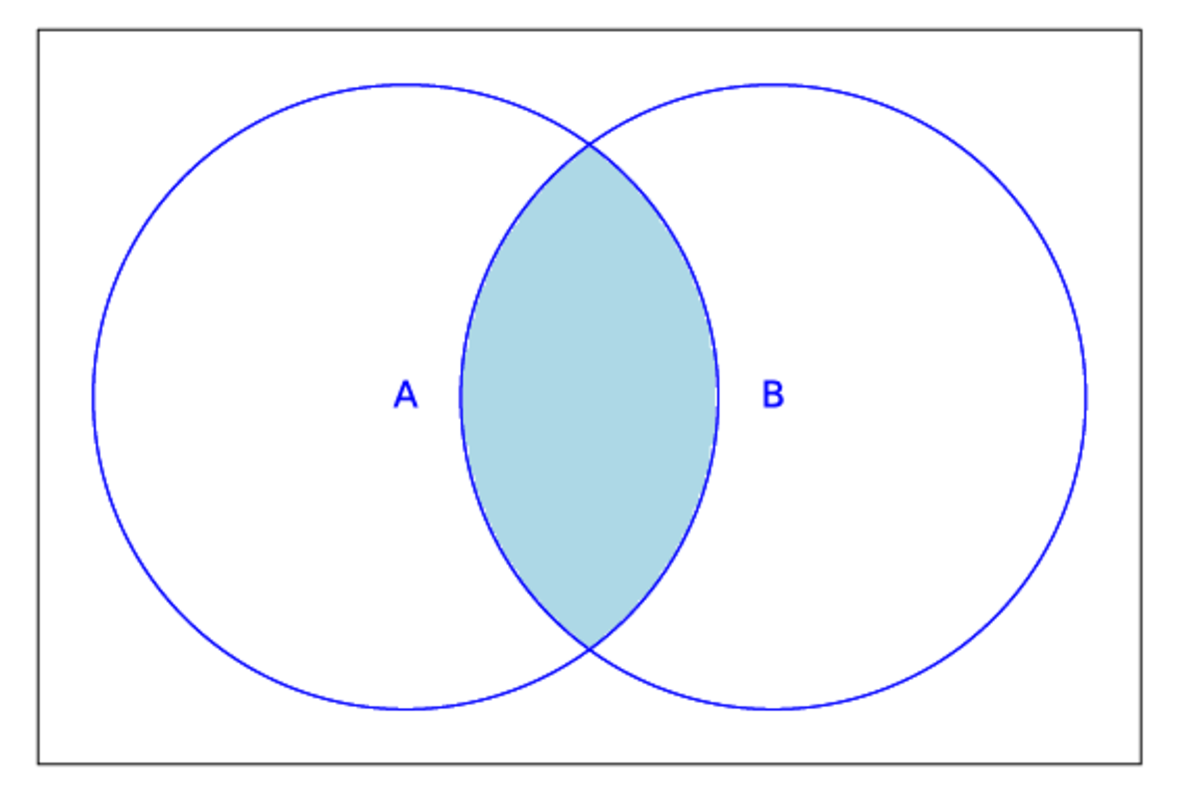
\includegraphics[width=1\linewidth]{images/sageplot-venn-intersection.pdf}}%
{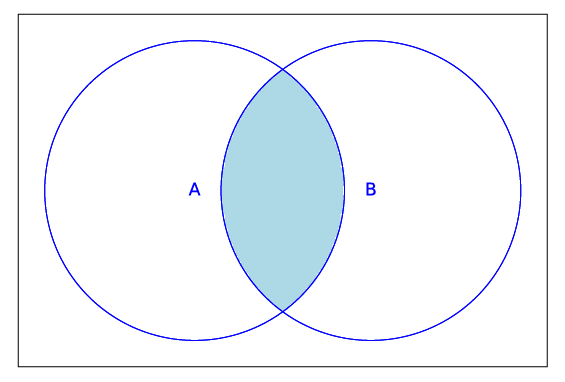
\includegraphics[width=1\linewidth]{images/sageplot-venn-intersection.png}}
\caption{Venn Diagram for the Intersection of Two Sets\label{venn_diagram_intersection}}
\end{figure}
\par
 The union \(A \cup  B\) is illustrated in \hyperref[venn_diagram_union]{\ref{venn_diagram_union}}.%
\leavevmode%
\begin{figure}
\centering
\IfFileExists{images/sageplot-venn-union.pdf}%
{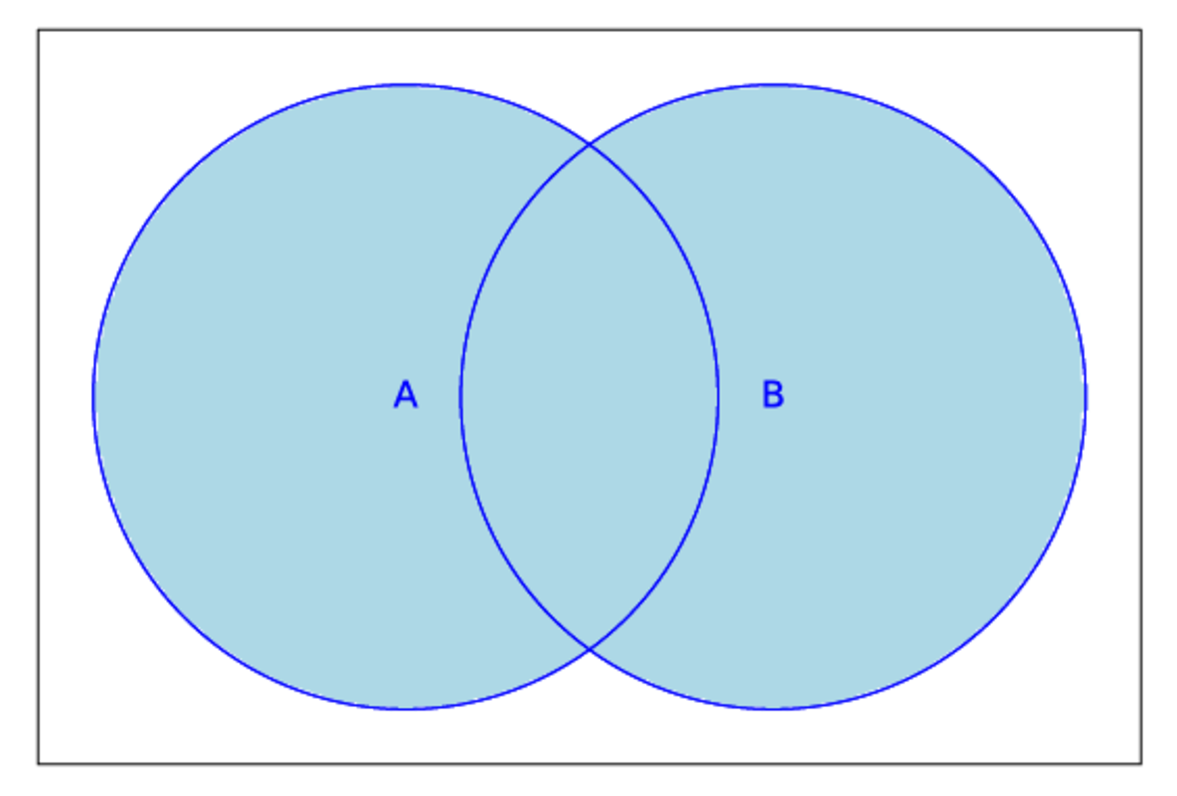
\includegraphics[width=1\linewidth]{images/sageplot-venn-union.pdf}}%
{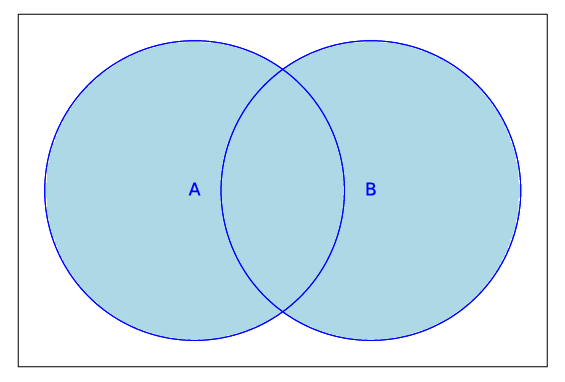
\includegraphics[width=1\linewidth]{images/sageplot-venn-union.png}}
\caption{Venn Diagram for the union \(A \cup  B\) \label{venn_diagram_union}}
\end{figure}
\par
In a Venn diagram, the region representing \(A \cap  B\) does not appear empty; however, in some instances it will represent the empty set. The same is true for any other region in a Venn diagram. 
%
\end{example}
\begin{definition}[Complement of a set]\label{set_complement.}
\index{Complement of a set}\label{notation-8}
\label{notation-9}
Let \( A\) and \( B\) be sets. The complement of \( A\) relative to \( B\) (notation
\(B - A\)) is the set of elements that are in \( B\) and not in \( A\). That is, \(B-A=\{x: x\in B \textrm{ and } x\notin A\}\). If \(
U\) is the universal set, then \(U-A\) is denoted by \(A^c\) and is called simply the complement of \( A\). \(A^c=\{x\in U : x\notin A\}\). 
%
\end{definition}
\begin{example}[Some Complements]\label{complements}
\leavevmode%
\begin{figure}
\centering
\IfFileExists{images/sageplot-venn-complement1.pdf}%
{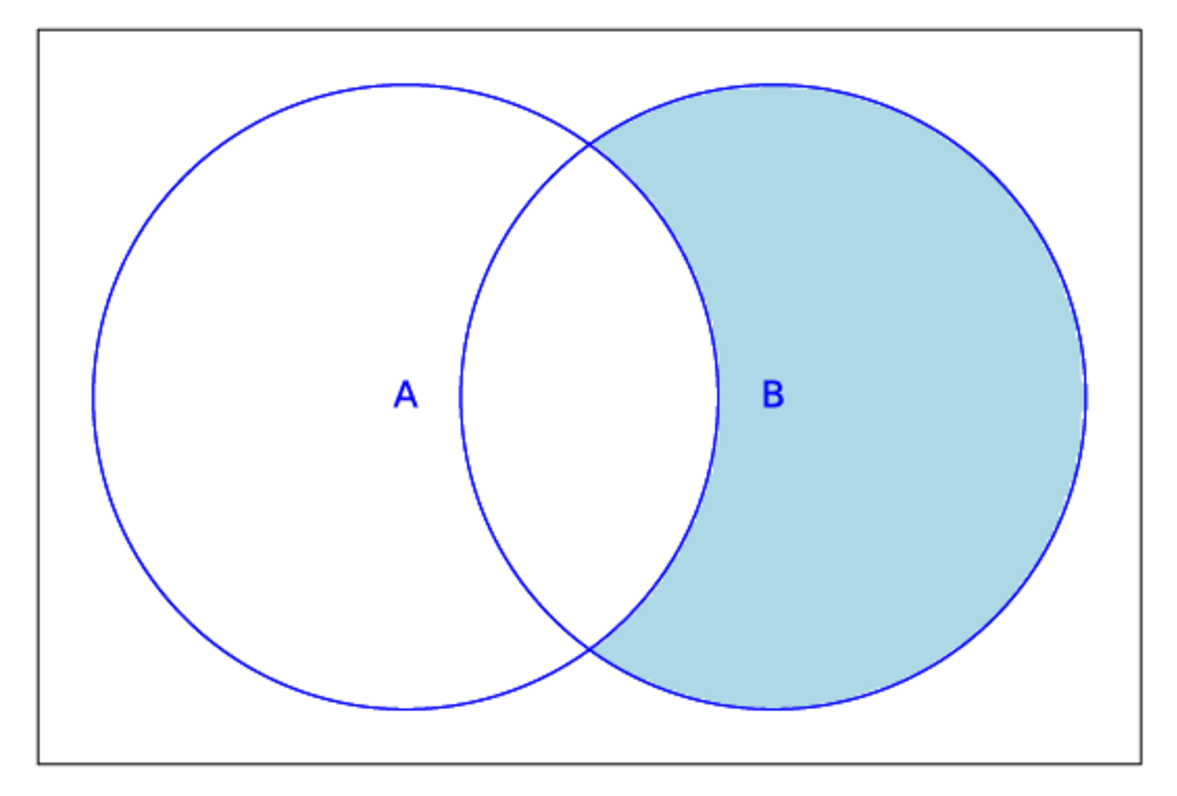
\includegraphics[width=1\linewidth]{images/sageplot-venn-complement1.pdf}}%
{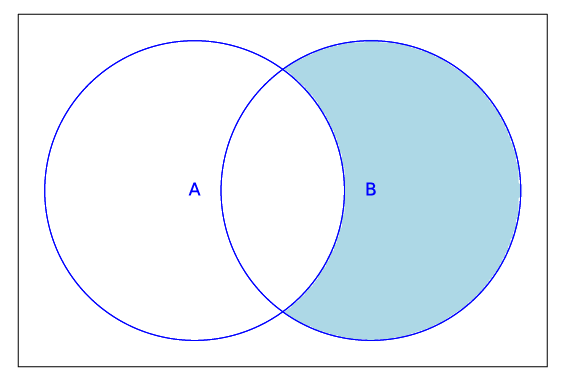
\includegraphics[width=1\linewidth]{images/sageplot-venn-complement1.png}}
\caption{Venn Diagram for \(B - A\)\label{venn_diagram_complement1}}
\end{figure}
\leavevmode%
\begin{enumerate}[label=\alph*]
\item\hypertarget{li-65}{} Let \(U = \{1,2, 3, \text{...} , 10\}\) and \(A = \{2,4,6,8, 10\}\). Then \(U-A = \{1, 3, 5, 7, 9\}\) and \(A - U= \emptyset\)%
\item\hypertarget{li-66}{} If \(U = \mathbb{R}\), then the complement of the rational numbers is the irrational numbers. 
%
\item\hypertarget{li-67}{}\(U^c= \emptyset\) and \(\emptyset ^c= U\). 
%
\item\hypertarget{li-68}{} The Venn diagram of \(B - A\) is represented in \hyperref[venn_diagram_complement1]{\ref{venn_diagram_complement1}}. %
\item\hypertarget{li-69}{} The Venn diagram of \(A^c\) is represented in \hyperref[venn_diagram_complement2]{\ref{venn_diagram_complement2}}. %
\item\hypertarget{li-70}{} If \(B\subseteq A\), then the Venn diagram of \(A- B\) is as shown in \hyperref[venn_diagram_complement3]{\ref{venn_diagram_complement3}}. %
\item\hypertarget{li-71}{} In the universe of integers, the set of even integers, \(\{\ldots  , - 4,-2, 0, 2, 4,\ldots \}\), has the set of odd integers as its complement.%
\end{enumerate}
%
\leavevmode%
\begin{figure}
\centering
\IfFileExists{images/sageplot-venn-complement2.pdf}%
{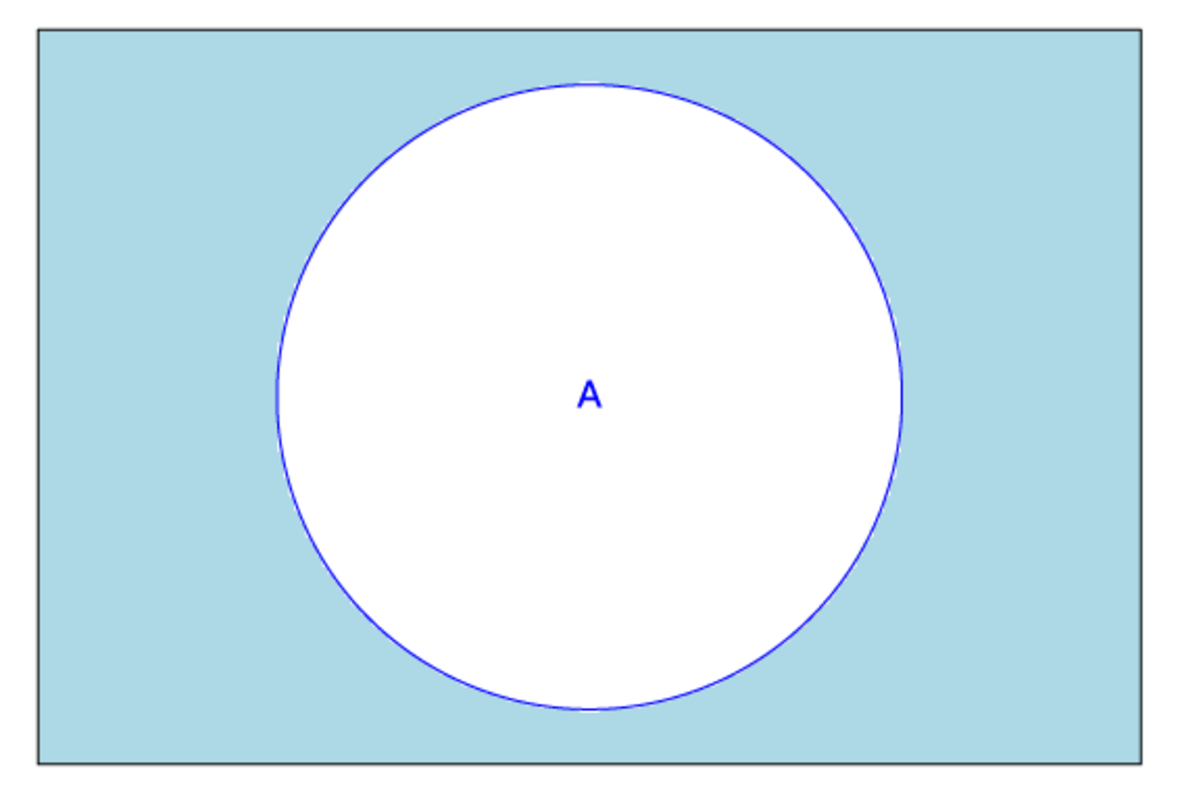
\includegraphics[width=1\linewidth]{images/sageplot-venn-complement2.pdf}}%
{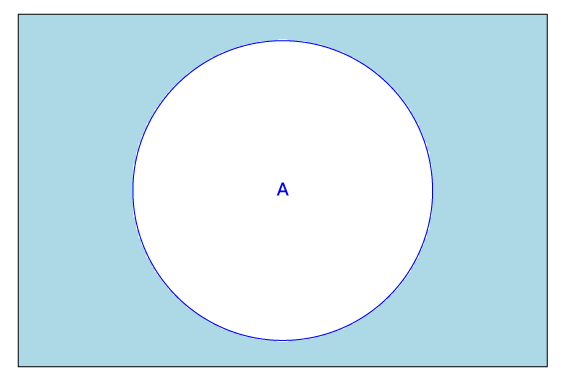
\includegraphics[width=1\linewidth]{images/sageplot-venn-complement2.png}}
\caption{Venn Diagram for \(A^{c}\)\label{venn_diagram_complement2}}
\end{figure}
\leavevmode%
\begin{figure}
\centering
\IfFileExists{images/sageplot-venn-complement3.pdf}%
{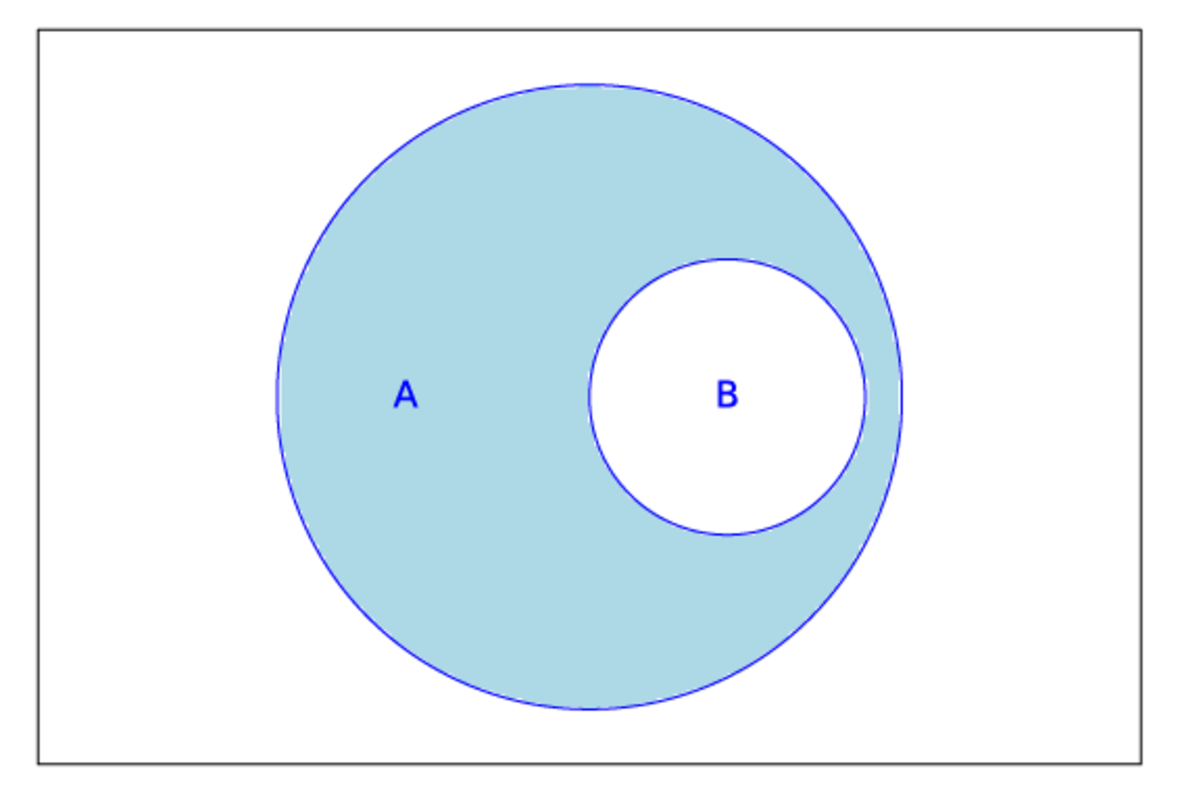
\includegraphics[width=1\linewidth]{images/sageplot-venn-complement3.pdf}}%
{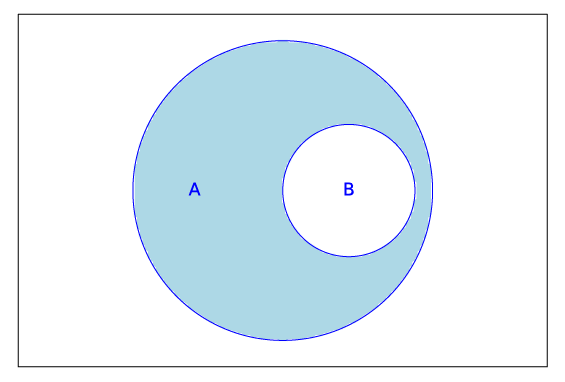
\includegraphics[width=1\linewidth]{images/sageplot-venn-complement3.png}}
\caption{Venn Diagram for \(A^{c}\)\label{venn_diagram_complement3}}
\end{figure}
\end{example}
\begin{definition}[ Symmetric Difference]\label{symmetric-difference.}
\index{Symmetric Difference}\label{notation-10}
Let A and B be sets. The symmetric difference of A and B (denoted by \(A\oplus B\)) is the set of all elements
that are in A and B but not in both. That is, \(A \oplus  B = (A \cup  B) - (A \cap  B)\). %
\end{definition}
\begin{example}[Some Symmetric Differences]\label{some_symmetric_differences}
\leavevmode%
\begin{enumerate}[label=\alph*]
\item\hypertarget{li-72}{}Let \(A = \{1, 3, 8\}\) and \(B = \{2, 4, 8\}\). Then \(A \oplus  B = \{1, 2, 3, 4\}\). 
%
\item\hypertarget{li-73}{}\(A \oplus  0 = A\) and \(A \oplus  A = \emptyset\) for any set \(A\). 
%
\item\hypertarget{li-74}{}\(\mathbb{R} \oplus  \mathbb{Q}\) is the set of irrational numbers. 
%
\item\hypertarget{li-75}{}The Venn diagram of \(A \oplus  B\) is represented in \hyperref[venn_diagram_symmetric]{\ref{venn_diagram_symmetric}}.%
\end{enumerate}
%
\leavevmode%
\begin{figure}
\centering
\IfFileExists{images/sageplot-venn-symmetric.pdf}%
{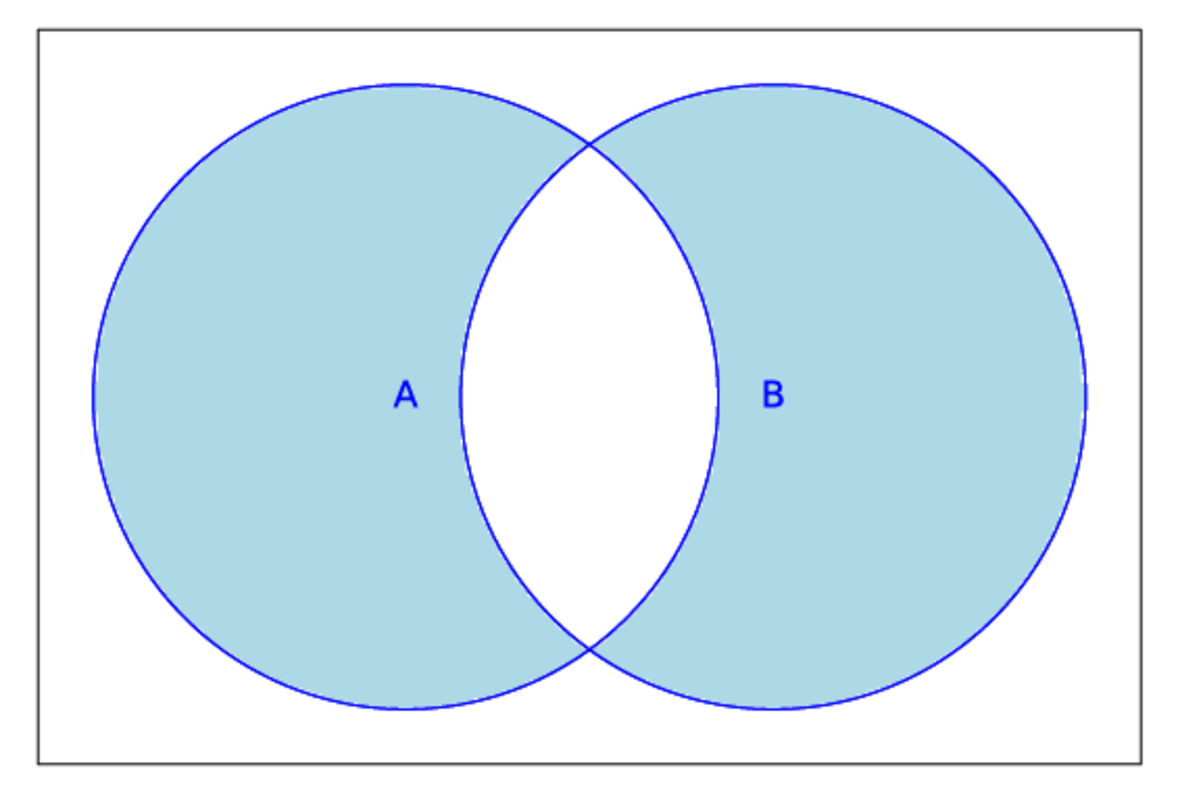
\includegraphics[width=1\linewidth]{images/sageplot-venn-symmetric.pdf}}%
{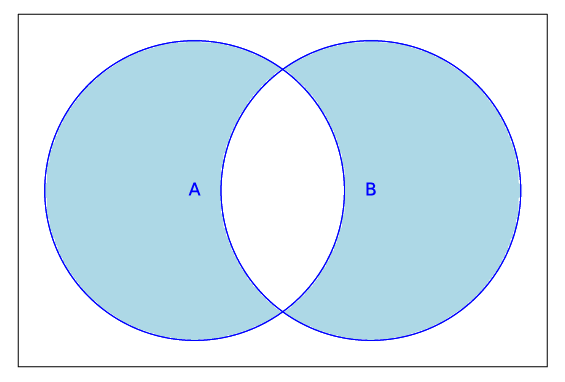
\includegraphics[width=1\linewidth]{images/sageplot-venn-symmetric.png}}
\caption{Venn Diagram for the symmetric difference \(A \oplus  B\)\label{venn_diagram_symmetric}}
\end{figure}
\end{example}
\typeout{************************************************}
\typeout{Subsection 1.2.3 Sage Note: Sets}
\typeout{************************************************}
\subsection[Sage Note: Sets]{Sage Note: Sets}\label{Sage_Note_Sets-1-2}
\index{Sage Note!Sets}To work with sets in Sage, a set is an expression of the form  Set(\emph{list}).  By wrapping a list with set, the order of elements appearing in the list and their duplication are ignored.  For example, L1 and L2 are two different lists, but notice how as sets they are considered equal:%
\begin{lstlisting}[style=sageinput]
L1=[3,6,9,0,3]
L2=[9,6,3,0,9]
[L1==L2, Set(L1)==Set(L2) ]
\end{lstlisting}
\begin{lstlisting}[style=sageoutput]
[False,True]
\end{lstlisting}
\par
The standard set operations are all methods and/or functions that can act on Sage sets. \emph{You need to evalute the following cell to use the subsequent cell.}%
\begin{lstlisting}[style=sageinput]
A=Set(srange(5,50,5))
B=Set(srange(6,50,6))
[A,B]
\end{lstlisting}
\begin{lstlisting}[style=sageoutput]
[{35, 5, 40, 10, 45, 15, 20, 25, 30}, {36, 6, 42, 12, 48, 18, 24, 30}]
\end{lstlisting}
\par

We can test membership, asking whether 10 is in each of the sets:
%
\begin{lstlisting}[style=sageinput]
[10 in A, 10 in B]
\end{lstlisting}
\begin{lstlisting}[style=sageoutput]
[True, False]
\end{lstlisting}
\par

The ampersand is used for the intersection of sets.  Change it to the vertical bar, |, for union. 
%
\begin{lstlisting}[style=sageinput]
A & B
\end{lstlisting}
\begin{lstlisting}[style=sageoutput]
{30}
\end{lstlisting}
\par
Symmetric difference and set complement are defined as ``methods'' in Sage. Here is how to compute the symmetric difference of \(A\)  with  \(B\), followed by their differences.%
\begin{lstlisting}[style=sageinput]
[A.symmetric_difference(B),A.difference(B),B.difference(A)]
\end{lstlisting}
\begin{lstlisting}[style=sageoutput]
[{35, 36, 5, 6, 40, 42, 12, 45, 15, 48, 18, 20, 24, 25, 10},
 {35, 5, 40, 10, 45, 15, 20, 25},
 {48, 18, 36, 6, 24, 42, 12}]
\end{lstlisting}
\typeout{************************************************}
\typeout{Exercises 1.2.4 EXERCISES FOR SECTION 1.2 }
\typeout{************************************************}
\subsection[EXERCISES FOR SECTION 1.2 ]{EXERCISES FOR SECTION 1.2 }\label{exercises-1.2}
\hypertarget{exercisegroup-3}{}\typeout{************************************************}
\typeout{Introduction  }
\typeout{************************************************}
A Exercises%
\begin{exercisegroup}
\item[1.]\hypertarget{exercise-7}{} Let \(A = \{0, 2, 3\}\), \(B = \{2, 3\}\), \(C = \{1, 5, 9\}\), and let the universal set be \(U = \{0, 1, 2, . . . , 9\}\). Determine: %
\par
\leavevmode%
\begin{multicols}{3}
\begin{enumerate}[label=\alph*]
\item\hypertarget{li-76}{}  \(A \cap  B\)  %
\item\hypertarget{li-77}{}  \(A \cup  B\)%
\item\hypertarget{li-78}{}  \(B \cup  A\)   %
\item\hypertarget{li-79}{}  \(A \cup  C\) %
\item\hypertarget{li-80}{}  \(A - B\)%
\item\hypertarget{li-81}{}  \(B - A\)%
\item\hypertarget{li-82}{}   \(A^c\) %
\item\hypertarget{li-83}{}   \(C^c\)%
\item\hypertarget{li-84}{}  \(A\cap C\)%
\item\hypertarget{li-85}{}   \(A\oplus B\) %
\end{enumerate}
\end{multicols}
%
\par\smallskip
\par\smallskip
\noindent\textbf{Answer.}\hypertarget{answer-4}{}\quad
\leavevmode%
\begin{multicols}{3}
\begin{enumerate}[label=\alph*]
\item\hypertarget{li-86}{} \(\{2,3\}\)%
\item\hypertarget{li-87}{} \(\{0,2,3\}\)%
\item\hypertarget{li-88}{} \(\{0,2,3\}\)%
\item\hypertarget{li-89}{}\(\{0,1,2,3,5,9\}\)%
\item\hypertarget{li-90}{}\(\{0\}\) %
\item\hypertarget{li-91}{} \(\emptyset\) %
\item\hypertarget{li-92}{}\(\{ 1,4,5,6,7,8,9\}\) %
\item\hypertarget{li-93}{} \(\{0,2,3,4,6,7,8\}\)%
\item\hypertarget{li-94}{} \(\emptyset\) %
\item\hypertarget{li-95}{} \(\{0\}\)%
\end{enumerate}
\end{multicols}
%
\item[2.]\hypertarget{exercise-8}{}  Let \( A\), \( B\), and \( C\) be as in Exercise 1, let \(D = \{3, 2\}\), and let \(E = \{2, 3, 2\}\). Determine which of the
following are true. Give reasons for your decisions. %
\par
\leavevmode%
\begin{multicols}{2}
\begin{enumerate}[label=\alph*]
\item\hypertarget{li-96}{}  \(A = B\) %
\item\hypertarget{li-97}{}  \(B = C\) %
\item\hypertarget{li-98}{}  \(B = D\) %
\item\hypertarget{li-99}{}  \(E=D\)%
\item\hypertarget{li-100}{}  \(A\cap B = B\cap A\)%
\item\hypertarget{li-101}{}  \(A \cup  B = B \cup  A\) %
\item\hypertarget{li-102}{}  \(A-B = B-A\) %
\item\hypertarget{li-103}{}  \(A \oplus  B = B \oplus  A\) %
\end{enumerate}
\end{multicols}
%
\par\smallskip
\item[3.]\hypertarget{exercise-9}{}  Let \(U= \{1, 2, 3, . . . , 9\}\). 
Give examples of sets \( A\), \( B\), and \( C\) for which:
%
\par
\leavevmode%
\begin{multicols}{2}
\begin{enumerate}[label=\alph*]
\item\hypertarget{li-104}{}  \(A\cap (B\cap C)=(A\cap B)\cap C\) %
\item\hypertarget{li-105}{}  \(A\cap (B\cup C)=(A\cap B)\cup (A\cap C)\)%
\item\hypertarget{li-106}{}  \((A \cup  B)^c= A^c\cap B^c\) %
\item\hypertarget{li-107}{}  \(A \cup  A^c = U\)%
\item\hypertarget{li-108}{}  \(A \subseteq A\cup B\)%
\item\hypertarget{li-109}{}  \(A\cap B \subseteq A\) %
\end{enumerate}
\end{multicols}
%
\par\smallskip
\par\smallskip
\noindent\textbf{Answer.}\hypertarget{answer-5}{}\quad
 These are all true for any sets \(A\), \(B\), and \(C\). %
\item[4.]\hypertarget{exercise-10}{} Let \(U= \{1, 2, 3, . . . , 9\}\). Give examples to illustrate the following facts: %
\par
\leavevmode%
\begin{multicols}{1}
\begin{enumerate}[label=\alph*]
\item\hypertarget{li-110}{}  If \(A \subseteq  B\) and \(B \subseteq C\), then \(A\subseteq C\).%
\item\hypertarget{li-111}{} There are sets \(A\) and \(B\) such that \(A - B \neq  B - A\) %
\item\hypertarget{li-112}{}  If \(U = A\cup  B\) and \(\text{A $\cap $ B = $\emptyset $}\), it always follows that \(A = U - B\). %
\item\hypertarget{li-113}{}  \(A \oplus  (B\cap C) = (A \oplus  B)\cap  (A \oplus C)\)   %
\end{enumerate}
\end{multicols}
%
\par\smallskip
\end{exercisegroup}
\par\smallskip\noindent
\hypertarget{exercisegroup-4}{}\typeout{************************************************}
\typeout{Introduction  }
\typeout{************************************************}
B Exercises%
\begin{exercisegroup}
\item[5.]\hypertarget{exercise-11}{}  What can you say about \(A\) if \(U = \{1, 2, 3, 4, 5\}\), \(B = \{2, 3\}\), and (separately) %
\par
\leavevmode%
\begin{multicols}{1}
\begin{enumerate}[label=\alph*]
\item\hypertarget{li-114}{}  \(A \cup B = \{1, 2, 3,4\}\) %
\item\hypertarget{li-115}{}  \(A \cap  B = \{2\}\) %
\item\hypertarget{li-116}{}  \(A \oplus  B = \{3, 4, 5\}\)%
\end{enumerate}
\end{multicols}
%
\par\smallskip
\par\smallskip
\noindent\textbf{Answer.}\hypertarget{answer-6}{}\quad
\leavevmode%
\begin{enumerate}[label=\alph*]
\item\hypertarget{li-117}{} \(\{1, 4\} \subseteq  A \subseteq  \{1, 2, 3, 4\}\)%
\item\hypertarget{li-118}{} \(\{2\} \subseteq  A \subseteq  \{1, 2, 4, 5\}\) %
\item\hypertarget{li-119}{} \(A = \{2, 4, 5\}\)%
\end{enumerate}
%
\item[6.]\hypertarget{exercise-12}{} Suppose that \( U\) is an infinite universal set, and \( A\) and \( B\) are infinite subsets of \( U\). Answer the following questions with a brief explanation.%
\par
\leavevmode%
\begin{multicols}{1}
\begin{enumerate}[label=\alph*]
\item\hypertarget{li-120}{}  Must \(A^c\) be finite? %
\item\hypertarget{li-121}{}  Must \(A\cup B\) infinite? %
\item\hypertarget{li-122}{}  Must \(A\cap B\) be infinite? %
\end{enumerate}
\end{multicols}
%
\par\smallskip
\item[7.]\hypertarget{exercise-13}{}  Given that \( U\) = all students at a university, \( D\) = day students, \( M\) = mathematics majors, and \( G\) = graduate students. Draw Venn diagrams illustrating this situation and shade in the following sets:%
\par
\leavevmode%
\begin{multicols}{2}
\begin{enumerate}[label=\alph*]
\item\hypertarget{li-123}{}  evening students %
\item\hypertarget{li-124}{}  undergraduate mathematics majors %
\item\hypertarget{li-125}{}  non-math graduate students %
\item\hypertarget{li-126}{}  non-math undergraduate students%
\end{enumerate}
\end{multicols}
%
\par\smallskip
\par\smallskip
\noindent\textbf{Answer.}\hypertarget{answer-7}{}\quad
\leavevmode%
\begin{figure}
\centering
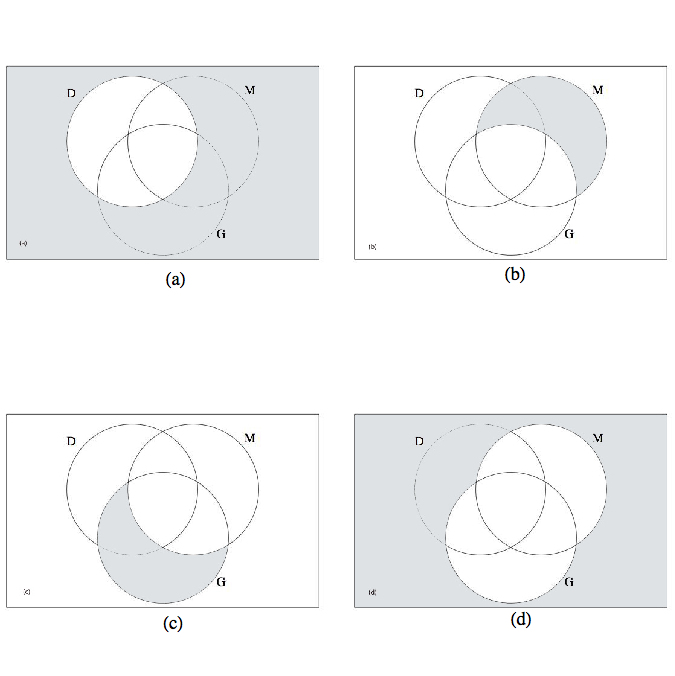
\includegraphics[width=1\linewidth]{images/fig-sol-1-2-7.png}
\caption{
	 \label{fig-sol-1-2-7}}
\end{figure}
\item[8.]\hypertarget{exercise-14}{} Let the sets \( D\), \( M\), \( G\), and \( U\) be as in exercise 7.  Let \(\lvert U \rvert  = 16,000\), \(\lvert D \rvert = 9,000\), \(|M |=
300\), and \(\lvert G \rvert = 1,000\). Also assume that the number of day students who are mathematics majors is 250, 50 of whom are graduate students, that there are 95 graduate mathematics majors, and that the total number of day graduate students is 700. Determine the number of students who are: %
\par
\leavevmode%
\begin{multicols}{2}
\begin{enumerate}[label=\alph*]
\item\hypertarget{li-127}{}  evening students %
\item\hypertarget{li-128}{}  nonmathematics majors %
\item\hypertarget{li-129}{}  undergraduates (day or evening) %
\item\hypertarget{li-130}{}  day graduate nonmathematics majors %
\item\hypertarget{li-131}{}  evening graduate students %
\item\hypertarget{li-132}{}  evening graduate mathematics majors %
\item\hypertarget{li-133}{}  evening undergraduate nonmathematics majors %
\end{enumerate}
\end{multicols}
%
\par\smallskip
\end{exercisegroup}
\par\smallskip\noindent
\typeout{************************************************}
\typeout{Section 1.3 Cartesian Products and Power Sets}
\typeout{************************************************}
\section[Cartesian Products and Power Sets]{Cartesian Products and Power Sets}\label{Cartesian_Products_and_Power_Sets}
\typeout{************************************************}
\typeout{Subsection 1.3.1 Cartesian Products}
\typeout{************************************************}
\subsection[Cartesian Products]{Cartesian Products}\label{Cartesian-products}
\begin{definition}[ Cartesian Product]\label{cartesian-product.}
\index{Cartesian Product}\label{notation-11}
 Let \(A\) and \(B\) be sets. The Cartesian product of \(A\) and \(B\), denoted by \(A\times B\), is defined as follows: \(A\times B = \{(a, b) \mid a \in  A \quad\textrm{ and }\quad b \in  B\}\), that is, \(A\times B\) is the set of all possible ordered pairs whose first component comes from \(A\) and whose second component comes from \(B\).%
\end{definition}
\begin{example}[Some Cartesian Products]\label{example-8}
 Notation in mathematics is often developed for good reason. In this case, a few examples will make clear why the symbol $\times $ is used for Cartesian products.%
\par
\leavevmode%
\begin{itemize}[label=\textbullet]
\item{}  Let \(A = \{1, 2, 3\}\) and \(B = \{4, 5\}\). Then \(A \times  B = \{(1, 4), (1, 5), (2, 4), (2, 5), (3, 4), (3, 5)\}\). Note that \(|A \times B| = 6 = \lvert A \rvert  \times  \lvert B \rvert \). %
\item{}  \(A \times  A = \{(1, 1), (1, 2), (1, 3), (2, 1), (2, 2), (2, 3), (3, 1), (3, 2), (3, 3)\}\). Note that \(|A \times  A| = 9 = {\lvert A \rvert}^2\).%
\end{itemize}
%
\end{example}
These two examples illustrate the general rule: If A and B are finite sets, then \(| A \times B | = \lvert A \rvert  \times  \lvert B \rvert \).%
\par
We can define the Cartesian product of three (or more) sets similarly. For example, \(A \times  B \times  C = \{(a, b, c):a \in  A, b \in  B, c \in C\}\). %
\par
It is common to use exponents if the sets in a Cartesian product are the same: 
\begin{equation*}A^2= A \times  A\end{equation*}
\begin{equation*}A^3=A \times A \times A\end{equation*}
and in general, 
\begin{equation*}A^n =  \underset{n \textrm{ factors}}{\underline{A \times A \times \ldots \times A}}\end{equation*}.%
\typeout{************************************************}
\typeout{Subsection 1.3.2 Power Sets}
\typeout{************************************************}
\subsection[Power Sets]{Power Sets}\label{power-sets}
\begin{definition}[ Power Set ]\label{power-set}
\index{Power Set }\label{notation-12}
If \( A\) is any set, the power set of \(A\) is the set of all subsets of \(A\), denoted \(\mathcal{P}(A)\).%
\end{definition}
The two extreme cases, the empty set and all of \(A\), are both included in \(\mathcal{P}(A)\).%
\begin{example}[ Some Power Sets ]\label{Some_Power_Sets}
\leavevmode%
\begin{itemize}[label=\textbullet]
\item{}\(\mathcal{P}(\emptyset )=\{\emptyset \}\) %
\item{} \(\mathcal{P}(\{1\}) = \{\emptyset , \{1\}\}\) %
\item{} \(\mathcal{P}(\{1,2\}) = \{\emptyset , \{1\}, \{2\}, \{1, 2\}\}\). %
\end{itemize}
%
\par
We will leave it to you to guess at a general formula for the number of elements in the power set of a finite set. In Chapter 2, we will discuss counting rules that will help us derive this formula.%
\end{example}
\typeout{************************************************}
\typeout{Subsection 1.3.3 Sage Note: Cartesion Products and Power Sets}
\typeout{************************************************}
\subsection[Sage Note: Cartesion Products and Power Sets]{Sage Note: Cartesion Products and Power Sets}\label{Sage_Note_Sets-1-3}
\index{Sage Note!Cartesion Products and Power Sets}Here is a simple example of a cartesion product of two sets:%
\begin{lstlisting}[style=sageinput]
A=Set([0,1,2])
B=Set(['a','b'])
P=cartesian_product([A,B]);P
\end{lstlisting}
\begin{lstlisting}[style=sageoutput]
The cartesian product of ({0, 1, 2}, {'a', 'b'})
\end{lstlisting}
\par
Here is the cardinality of the cartesian product.%
\begin{lstlisting}[style=sageinput]
P.cardinality()
\end{lstlisting}
\begin{lstlisting}[style=sageoutput]
6
\end{lstlisting}
\par

The power set of a set is an iterable, as you can see from the output of this next cell
%
\begin{lstlisting}[style=sageinput]
U=Set([0,1,2,3])
subsets(U)
\end{lstlisting}
\begin{lstlisting}[style=sageoutput]
<generator object powerset at 0x7fec5ffd33c0>
\end{lstlisting}
\par

You can iterate over a powerset - here is a trivial example.  
%
\begin{lstlisting}[style=sageinput]
for a in subsets(U):
    print(str(a)+ " has " +str(len(a))+" elements.")
\end{lstlisting}
\begin{lstlisting}[style=sageoutput]
[] has 0 elements.
[0] has 1 elements.
[1] has 1 elements.
[0, 1] has 2 elements.
[2] has 1 elements.
[0, 2] has 2 elements.
[1, 2] has 2 elements.
[0, 1, 2] has 3 elements.
[3] has 1 elements.
[0, 3] has 2 elements.
[1, 3] has 2 elements.
[0, 1, 3] has 3 elements.
[2, 3] has 2 elements.
[0, 2, 3] has 3 elements.
[1, 2, 3] has 3 elements.
[0, 1, 2, 3] has 4 elements.
\end{lstlisting}
\typeout{************************************************}
\typeout{Exercises 1.3.4 EXERCISES FOR SECTION 1.3 }
\typeout{************************************************}
\subsection[EXERCISES FOR SECTION 1.3 ]{EXERCISES FOR SECTION 1.3 }\label{exercises-1.3}
\hypertarget{exercisegroup-5}{}\typeout{************************************************}
\typeout{Introduction  }
\typeout{************************************************}
A Exercises%
\begin{exercisegroup}
\item[1.]\hypertarget{exercise-15}{} Let \(A = \{0, 2, 3\}\), \(B = \{2, 3\}\), \(C = \{1, 4\}\), and let the universal set be \(U = \{0, 1, 2, 3, 4\}\). List the elements of %
\par
\leavevmode%
\begin{multicols}{2}
\begin{enumerate}[label=\alph*]
\item\hypertarget{li-139}{}  \(A \times B\) %
\item\hypertarget{li-140}{}  \(B \times  A\) %
\item\hypertarget{li-141}{}  \(A \times B\times C\) %
\item\hypertarget{li-142}{}  \(U \times \emptyset\)%
\item\hypertarget{li-143}{}  \(A \times  A^c\)%
\item\hypertarget{li-144}{}  \(B^2\) %
\item\hypertarget{li-145}{}  \(B^3\)%
\item\hypertarget{li-146}{}  \(B\times \mathcal{P}(B)\)%
\end{enumerate}
\end{multicols}
%
\par\smallskip
\par\smallskip
\noindent\textbf{Answer.}\hypertarget{answer-8}{}\quad
\leavevmode%
\begin{enumerate}[label=\alph*]
\item\hypertarget{li-147}{} \(\{(0, 2), (0, 3), (2, 2), (2, 3), (3, 2), (3, 3)\}\)%
\item\hypertarget{li-148}{}\(\{(2, 0), (2, 2), (2, 3), (3, 0), (3, 2), (3, 3)\}\)%
\item\hypertarget{li-149}{} \(\{(0, 2, 1), (0, 2, 4), (0, 3, 1), (0, 3, 4), (2, 2, 1), (2, 2, 4),\\ (2, 3, 1), (2, 3, 4), (3, 2, 1), (3, 2, 4), (3, 3, 1), (3, 3, 4)\}\)%
\item\hypertarget{li-150}{}\(\emptyset\)%
\item\hypertarget{li-151}{} \(\{(0, 1), (0, 4), (2, 1), (2, 4), (3, 1), (3, 4)\}\)%
\item\hypertarget{li-152}{}\(\{(2, 2), (2, 3), (3, 2), (3, 3)\}\)%
\item\hypertarget{li-153}{} \(\{(2, 2, 2), (2, 2, 3), (2, 3, 2), (2, 3, 3), (3, 2, 2), (3, 2, 3), (3, 3, 2), (3, 3, 3)\}\)%
\item\hypertarget{li-154}{} \(\{(2, \emptyset ), (2, \{2\}), (2, \{3\}), (2, \{2, 3\}), (3, \emptyset ), (3, \{2\}), (3, \{3\}), (3, \{2, 3\})\}\)%
\end{enumerate}
%
\item[2.]\hypertarget{exercise-16}{} 
Suppose that you are about to flip a coin and then roll a die. Let \(A = \{HEADS, TAILS\}\) and  \(B = {$1, 2, 3, 4, 5, 6}\). %
\par
\leavevmode%
\begin{itemize}[label=\textbullet]
\item{}  What is \(|A \times  B|\)? %
\item{}  How could you interpret the set \(A \times  B\) ?   %
\end{itemize}
%
\par\smallskip
\item[3.]\hypertarget{exercise-17}{} 
List all two-element sets in \(\mathcal{P}(\{a,b,c,d\})\) %
\par\smallskip
\par\smallskip
\noindent\textbf{Answer.}\hypertarget{answer-9}{}\quad
\(\{a, b\}, \{a, c\}, \{a, d\}, \{b, c\}, \{b, d\} and \{c, d\}\)%
\item[4.]\hypertarget{exercise-18}{}
List all three-element sets in \(\mathcal{P}(\{a, b, c,d\})\).%
\par\smallskip
\item[5.]\hypertarget{exercise-19}{}How many singleton (one-element) sets are there in \(\mathcal{P}(A)\) if \(\lvert A \rvert =n\) ? %
\par\smallskip
\par\smallskip
\noindent\textbf{Answer.}\hypertarget{answer-10}{}\quad
 There are \(n\) singleton subsets, one for each element.%
\item[6.]\hypertarget{exercise-20}{}A person has four coins in his pocket: a penny, a nickel, a dime, and a quarter. How many different sums of money can he take out if he removes 3 coins at a time? %
\par\smallskip
\item[7.]\hypertarget{exercise-21}{}Let \(A = \{+,-\}\) and \(B = \{00, 01, 10, 11\}\).%
\par
\leavevmode%
\begin{itemize}[label=\textbullet]
\item{}  List the elements of \(A \times  B\) %
\item{}  How many elements do \(A ^4\) and \((A \times B)^3\) have? %
\end{itemize}
%
\par\smallskip
\par\smallskip
\noindent\textbf{Answer.}\hypertarget{answer-11}{}\quad
\leavevmode%
\begin{enumerate}[label=\alph*]
\item\hypertarget{li-159}{} \(\{+00, +01, +10, +11, -00, -01, -10, -11\}\)%
\item\hypertarget{li-160}{} \(16 \textrm{ and } 512\)%
\end{enumerate}
%
\end{exercisegroup}
\par\smallskip\noindent
\hypertarget{exercisegroup-6}{}\typeout{************************************************}
\typeout{Introduction  }
\typeout{************************************************}
B Exercises%
\begin{exercisegroup}
\item[8.]\hypertarget{exercise-22}{}Let \(A = \{\bullet,\square ,\otimes \}\) and \(B = \{\square ,\ominus ,\bullet\}\). %
\par
\leavevmode%
\begin{itemize}[label=\textbullet]
\item{} List the elements of \(A \times  B\) and \(B \times  A\). The parentheses and comma in an ordered pair are not necessary in cases such as this where the elements of each set are individual symbols. %
\item{}  Identify the intersection of \(A \times  B\) and \(B \times  A\) for the case above, and then guess at a general rule for the intersection of \(A \times  B\) and \(B \times  A\). where \( A\) and \( B\) are any two sets. %
\end{itemize}
%
\par\smallskip
\item[9.]\hypertarget{exercise-23}{}Let \(A\) and \(B\) be nonempty sets. When are \(A \times  B\) and \(B \times  A\) equal? %
\par\smallskip
\par\smallskip
\noindent\textbf{Answer.}\hypertarget{answer-12}{}\quad
 They are equal when \(A=B\).%
\end{exercisegroup}
\par\smallskip\noindent
\typeout{************************************************}
\typeout{Section 1.4 Binary Representation of Positive Integers }
\typeout{************************************************}
\section[Binary Representation of Positive Integers ]{Binary Representation of Positive Integers }\label{Binary_Representation_of_Positive_Integers}
\index{Binary Representation}Recall that the set of positive integers, \(\mathbb{P}\), is \(\{1, 2, 3, . . . \}\). Positive integers are naturally used to count things. There are many ways to count and many ways to record, or represent, the results of counting. For example, if we wanted to count five hundred twenty-three apples, we might group the apples by tens. There would be fifty-two groups of ten with three single apples left over. The fifty-two groups of ten could be put into five groups of ten tens (hundreds), with two tens left over. The five hundreds, two tens, and three units is recorded as 523. This system of counting is called the base ten positional system, or decimal system. It is quite natural for us to do grouping by tens, hundreds, thousands, \(\dots\) since it is the method that all of us use in everyday life. %
\par
 The term positional refers to the fact that each digit in the decimal representation of a number has a significance based on its position. Of course this means that rearranging digits will change the number being described. You may have learned of numeraton systems in which the position of symbols does not have any significance (e.g., the ancient Egyptian system). Most of these systems are merely curiosities to us now.%
\par
The binary number system differs from the decimal number system in that units are grouped by twos, fours, eights, etc. That is, the group sizes are powers of two instead of powers of ten. For example, twenty-three can be grouped into eleven groups of two with one left over. The eleven twos can be grouped into five groups of four with one group of two left over. Continuing along the same lines, we find that twenty-three can be described as one sixteen, zero eights, one four, one two, and one one, which is abbreviated \(10111_{\textrm{two}}\), or simply \(10111\) if the
context is clear. %
\par
The process that we used to determine the binary representation of \(23\) can be described in general terms to determine the binary representation of any positive integer \(n\). A general description of a process such as this one is called an algorithm. Since this is the first algorithm in the book, we will first write it out using less formal language than usual, and then introduce some ``algorithmic notation.''  If you are unfamiliar with algorithms, we refer you to {$\langle\langle$Unresolved xref, reference "app-alg1"; check spelling or use "provisional" attribute$\rangle\rangle$}%
\par
\leavevmode%
\begin{enumerate}[label=\arabic*]
\item\hypertarget{li-163}{} Start with an empty list of bits. %
\item\hypertarget{li-164}{} Step Two: Assign the variable \(k\) the value \(n\). %
\item\hypertarget{li-165}{} Step Three: While \(k\)'s value is positive, continue performing the following three steps until \(k\) becomes zero and then stop. %
\par
%
\begin{enumerate}[label=\alph*]
\item\hypertarget{li-166}{}divide \(k\) by 2, obtaining a quotient \(q\) (often denoted \(k \textrm{ div } 2\)) and a remainder \(r\) (denoted \((k \bmod 2)\)). %
\item\hypertarget{li-167}{}attach \(r\) to the left-hand side of the list of bits. %
\item\hypertarget{li-168}{} assign the variable \(k\) the value \(q\).%
\end{enumerate}
%
\end{enumerate}
%
\begin{example}[An example of conversion to binary]\label{An_example_of_conversion_to_binary}
 To determine the binary representation of 41 we take the following steps:%
\par
\leavevmode%
\begin{itemize}[label=\textbullet]
\item{}\(41 = 2 \times  20+ 1 \quad List = 1 \) %
\item{}\(20 = 2 \times  10+0 \quad List = 01 \)%
\item{} \(10 = 2\times 5 + 0 \quad List = 001 \)%
\item{}\(5 =\text2\times  2+ 1 \quad List =1001\) %
\item{}\(2 =2\times  1+ 0 \quad List = 01001 \)%
\item{}\(1 =\text2 \times 0\text+1  \quad List = 101001\) %
\end{itemize}
%
\par
Therefore, \(41=101001_{\textrm{two}}\)%
\end{example}
\par
The notation that we will use to describe this algorithm and all others is called pseudocode, an informal variation of the instructions that are commonly used in many computer languages. Read the following description carefully, comparing it with the informal description above. Appendix B, which contains a general discussion of the components of the algorithms in this book, should clear up any lingering questions. Anything after // are comments.%
\begin{algorithm}[Binary Conversion Algorithm]\label{binary_conversion_algorithm}
\index{Binary Conversion Algorithm} An algorithm for determining the binary representation of a positive integer.%
\par
Input: a positive integer n.%
\par
Output: the binary representation of n in the form of a list of bits, with units bit last, twos bit next to last, etc.%
\par
\leavevmode%
\begin{enumerate}[label=\arabic*]
\item\hypertarget{li-175}{}k := n \(\qquad  \)     //initialize k%
\item\hypertarget{li-176}{}L := { } \(\qquad  \)   //initialize L to an empty list%
\item\hypertarget{li-177}{} While k > 0 do %
\par
%
\begin{enumerate}[label=\alph*]
\item\hypertarget{li-178}{} q := k div 2		\(\qquad  \)	//divide k by 2%
\item\hypertarget{li-179}{} r:= k mod 2 %
\item\hypertarget{li-180}{}L: = prepend r to L \(\qquad  \) //Add r to the front of L %
\item\hypertarget{li-181}{} k:= q   			\(\qquad  \)	//reassign k%
\end{enumerate}
%
\end{enumerate}
%
\end{algorithm}
\par
Here is a Sage version of the algorithm with two alterations. It outputs a the binary representation as a string, and it handles all integers, not just positive ones.%
\begin{lstlisting}[style=sageinput]
def binary_rep(n):
    if n==0:
        return '0'
    else:
        k=abs(n)
        s=''
        while k>0:
            s=str(k%2)+s
            k=k//2
        if n < 0:
            s='-'+s
        return s
 
binary_rep(41)
\end{lstlisting}
\begin{lstlisting}[style=sageoutput]
'101001'
\end{lstlisting}
\par
Now that you've read this section, you should get this joke.%
\leavevmode%
\begin{figure}
\centering
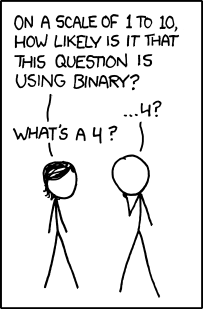
\includegraphics[width=1\linewidth]{images/1_to_10.png}
\caption{With permission from Randall Munroe
                \label{onetoten}}
\end{figure}
\typeout{************************************************}
\typeout{Exercises 1.4.1 EXERCISES}
\typeout{************************************************}
\subsection[EXERCISES]{EXERCISES}\label{exercises-1-4}
\hypertarget{exercisegroup-7}{}\typeout{************************************************}
\typeout{Introduction  }
\typeout{************************************************}
A Exercises%
\begin{exercisegroup}
\item[1.]\hypertarget{exercise-24}{}Find the binary representation of each of the following positive integers by working through the algorithm by hand.  You can check your answer using the sage cell above. %
\par
\leavevmode%
\begin{multicols}{2}
\begin{enumerate}[label=\alph*]
\item\hypertarget{li-182}{} 31%
\item\hypertarget{li-183}{} 32%
\item\hypertarget{li-184}{}10%
\item\hypertarget{li-185}{}100 %
\end{enumerate}
\end{multicols}
%
\par\smallskip
\par\smallskip
\noindent\textbf{Answer.}\hypertarget{answer-13}{}\quad
\leavevmode%
\begin{multicols}{2}
\begin{enumerate}[label=\alph*]
\item\hypertarget{li-186}{} \(11111\)%
\item\hypertarget{li-187}{} \(100000\)%
\item\hypertarget{li-188}{} \(1010\)%
\item\hypertarget{li-189}{} \(1100100\)%
\end{enumerate}
\end{multicols}
%
\item[2.]\hypertarget{exercise-25}{}Find the binary representation of each of the following positive integers by working through the algorithm by hand.  You can check your answer using the sage cell above. %
\par
\leavevmode%
\begin{multicols}{2}
\begin{enumerate}[label=\alph*]
\item\hypertarget{li-190}{} 64%
\item\hypertarget{li-191}{} 67%
\item\hypertarget{li-192}{}28%
\item\hypertarget{li-193}{}256 %
\end{enumerate}
\end{multicols}
%
\par\smallskip
\item[3.]\hypertarget{exercise-26}{}What positive integers have the following binary representations?%
\par
\leavevmode%
\begin{multicols}{2}
\begin{enumerate}[label=\alph*]
\item\hypertarget{li-194}{} 10010%
\item\hypertarget{li-195}{} 10011%
\item\hypertarget{li-196}{}101010%
\item\hypertarget{li-197}{}10011110000 %
\end{enumerate}
\end{multicols}
%
\par\smallskip
\par\smallskip
\noindent\textbf{Answer.}\hypertarget{answer-14}{}\quad
\leavevmode%
\begin{multicols}{2}
\begin{enumerate}[label=\alph*]
\item\hypertarget{li-198}{} \(18\)%
\item\hypertarget{li-199}{} \(19\)%
\item\hypertarget{li-200}{} \(42\)%
\item\hypertarget{li-201}{} \(1264\)%
\end{enumerate}
\end{multicols}
%
\item[4.]\hypertarget{exercise-27}{}What positive integers have the following binary representations?%
\par
\leavevmode%
\begin{multicols}{2}
\begin{enumerate}[label=\alph*]
\item\hypertarget{li-202}{} 100001%
\item\hypertarget{li-203}{} 1001001%
\item\hypertarget{li-204}{}1000000000%
\item\hypertarget{li-205}{}1001110000 %
\end{enumerate}
\end{multicols}
%
\par\smallskip
\item[5.]\hypertarget{exercise-28}{}The number of bits in the binary representations of integers increase by one as the numbers double.  Using this fact, determine how many bits the binary representations of the following decimal numbers have without actually doing the full conversion. 
\( \quad (a) 2017  \quad (b)  4000   \quad (c) 4500   \quad (d) 2^{50}\)%
\par\smallskip
\par\smallskip
\noindent\textbf{Answer.}\hypertarget{answer-15}{}\quad
There is a bit for each power of 2 up to the largest one needed to represent an integer, and you start counting with the zeroth power. For example, 2017 is between \(2^{10}=1024\) and \(2^{11}=2048\), and so the largest power needed is \(2^{10}\). Therefore there are \(11\) bits in binary 2017%
\par
\leavevmode%
\begin{multicols}{2}
\begin{enumerate}[label=\alph*]
\item\hypertarget{li-206}{} \(11\)%
\item\hypertarget{li-207}{} \(12\)%
\item\hypertarget{li-208}{} \(13\)%
\item\hypertarget{li-209}{} 51%
\end{enumerate}
\end{multicols}
%
\end{exercisegroup}
\par\smallskip\noindent
\hypertarget{exercisegroup-8}{}\typeout{************************************************}
\typeout{Introduction  }
\typeout{************************************************}
B Exercises%
\begin{exercisegroup}
\item[6.]\hypertarget{exercise-29}{}Let \(m\) be a positive integer with \( n\)-bit binary representation: \(a_{n-1}a_{n-2}\cdots  a_1a_0\) with \(a_{n-1}=1\) What are the smallest
and largest values that \(m\) could have? %
\par\smallskip
\item[7.]\hypertarget{exercise-30}{}If a positive integer is a multiple of 100, we can identify this fact from its decimal representation, since it will end with two zeros. What can you say about a positive integer if its binary representation ends with two zeros? What if i ends in \(k\) zeros?%
\par\smallskip
\par\smallskip
\noindent\textbf{Answer.}\hypertarget{answer-16}{}\quad
A number must be a multiple of four if its binary representation ends in two zeros. If it ends in \(k\) zeros, it must be a multiple of \(2^k\).%
\item[8.]\hypertarget{exercise-31}{}Can a multiple of ten be easily identified from its binary representation? %
\par\smallskip
\end{exercisegroup}
\par\smallskip\noindent
\typeout{************************************************}
\typeout{Section 1.5 Summation Notation and Generalizations }
\typeout{************************************************}
\section[Summation Notation and Generalizations ]{Summation Notation and Generalizations }\label{Summation_Notation_and_Generalizations}
\index{Summation Notation and Generalizations }Most operations such as addition of numbers are introduced as binary operations. That is, we are taught that two numbers may be added
together to give us a single number. Before long, we run into situations where more than two numbers are to be added. For example, if four numbers,
\(a_1\), \(a_2\), \(a_3\), and \(a_4\) are to be added, their sum may be written down in several ways, such as\(\) \(((a_1+a_2)+a_3)+a_4\)
or \(\left(a_1+a_2\right)+\left(a_3+a_4\right)\). In the first expression, the first two numbers are added, the result is added to the third number,
and that result is added to the fourth number. In the second expression the first two numbers and the last two numbers are added and the results
of these additions are added. Of course, we know that the final results will be the same. This is due to the fact that addition of numbers is an
associative operation. For such operations, there is no need to describe how more than two objects will be operated on. 
A sum of numbers such as \(a_1+a_2+a_3+a_4\)is called a series and is often written \(\sum _{k=1}^4 a_k\) in what is called \emph{ summation notation}. %
\par
We first recall some basic facts about series that you probably have seen before. A more formal treatment of sequences and series is covered in Chapter 8. The purpose here is to give the reader a working knowledge of summation notation and to carry this notation through to intersection
and union of sets and other mathematical operations. %
\par
A \emph{finite series} is an expression such as \(a_1+a_2+a_3 +\dots +a_n=\sum _{k=1}^{n} a_k\)%
\par
In the expression \(\sum _{k=1}^{n} a_k\):%
\par
\leavevmode%
\begin{itemize}[label=\textbullet]
\item{} The variable \(k\) is referred to as the \emph{ index}, or the index of summation.%
\item{} The expression \(a_k\) is the \emph{ general term} of the series. It defines the numbers that are being added together in the series.%
\item{} The value of \(k\) below the summation symbol is the \emph{ initial index} and the value above the summation symbol is the \emph{ terminal index}.%
\item{} It is understood that the series is a sum of the general terms where the index start with the initial index and increases by one up to and including the terminal index.%
\end{itemize}
%
\begin{example}[Some finite series]\label{some_finite_series}
(a)  \(\sum _{i=1}^4 a_i= a_1+ a_2+a_3+a_4\)%
\par
(b) \(\sum _{k=0}^5 b_k=b_0+b_1+b_2+b_3+b_4+b_5\)%
\par
(c) \(\sum _{i=-2}^2 c_i=c_{-2}+c_{-1}+c_0+c_1+c_2\)%
\end{example}
\begin{example}[More finite series ]\label{more_finite_series}
If the general terms in a series are more specific, the sum can often be simplified. For example,%
\par
\leavevmode%
\begin{enumerate}[label=\alph*]
\item\hypertarget{li-214}{} \(\sum _{i=1}^4 i^2=1^2+2^2+3^2+4^2=30\) %
\item\hypertarget{li-215}{}\begin{equation*}\begin{split}
	\sum _{i=1}^5 (2i-1)&=(2\ 1-1)+(2\ 2-1)+(2\ 3-1)+(2\ 4-1)+(2\ 5-1)\\
    & =1+3+5+7+9\\
    & =25\\
    /end{split}
    \end{equation*}%
\end{enumerate}
%
\end{example}
\par
Summation notation can be generalized to many mathematical operations, for example, 
\(A_1\cap A_2\cap A_3\cap A_4=\underset{i=1}{\overset{4}{\cap }}A_i\) %
\begin{definition}[Generalized Set Operations]\label{generalized-set-operations}
\index{Generalized Set Operations}Let \(A_1, A_2, \ldots , A_n\) be sets. Then: %
\par
\leavevmode%
\begin{enumerate}[label=\alph*]
\item\hypertarget{li-216}{}  \(A_1\cap A_2\cap \cdots \cap A_n=\underset{i=1}{\overset{n}{\cap }}A_i\)%
\item\hypertarget{li-217}{}   \(A_1\cup A_2\cup \cdots \cup A_n=\underset{i=1}{\overset{n}{\cup }}A_i\)%
\item\hypertarget{li-218}{}   \(A_1\times A_2\times \cdots \times A_n=\underset{i=1}{\overset{n}{\times }}A_i\)%
\item\hypertarget{li-219}{}   \(A_1\oplus A_2\oplus \cdots \oplus A_n=\underset{i=1}{\overset{n}{\oplus }}A_i\)%
\end{enumerate}
%
\end{definition}
\begin{example}[Some generalized operations]\label{some_generalized_operations}
If \(A_1 = \{0, 2, 3\}\), \(A_2 = \{1, 2, 3, 6\}\), and \(A_3 = \{-1, 0, 3, 9\}\), then 
 \begin{equation*}\underset{i=1}{\overset{3}{\cap }}A_i=A_1\cap A_2\cap A_3=\{3\}\end{equation*}
and
\begin{equation*}\underset{i=1}{\overset{3}{\cup }}A_i=A_1\cup A_2\cup A_3=\{-1,0,1,2,3,6,9\}\end{equation*}
With this notation it is quite easy to write lengthy expressions in a fairly compact form. For example, the statement 
    \begin{equation*}A\cap \left(B_1\cup B_2\cup \cdots \cup B_n\right)= \left(A\cap B_1\right)\cup \left(A\cap B_2\right)\cup \cdots \cup \left(A\cap
B_n\right)\end{equation*}
becomes 
   \begin{equation*}A \cap \left(\underset{i=1}{\overset{n}{\cup }}B_i\right)= \underset{i=1}{\overset{n}{\cup }}\left(A\cap B_i\right)\end{equation*}%
\end{example}
\typeout{************************************************}
\typeout{Exercises 1.5.1 Exercises}
\typeout{************************************************}
\subsection[Exercises]{Exercises}\label{exercises-1-5}
\hypertarget{exercisegroup-9}{}\typeout{************************************************}
\typeout{Introduction  }
\typeout{************************************************}
A Exercises%
\begin{exercisegroup}
\item[1.]\hypertarget{exercise-32}{}Calculate the following series:%
\par
\leavevmode%
\begin{multicols}{2}
\begin{enumerate}[label=\alph*]
\item\hypertarget{li-220}{}  \(\sum _{i=1}^3 (2 + 3i)\)%
\item\hypertarget{li-221}{}  \(\sum _{i=-2}^1 i^2\) %
\item\hypertarget{li-222}{}  \(\sum _{j=0}^n 2^j\text{   }\) for \(n= 1, 2, 3, 4\)%
\item\hypertarget{li-223}{}  \(\sum _{k=1}^n (2k-1)\) for \(n = 1, 2, 3, 4\) %
\end{enumerate}
\end{multicols}
%
\par\smallskip
\par\smallskip
\noindent\textbf{Answer.}\hypertarget{answer-17}{}\quad
\leavevmode%
\begin{multicols}{2}
\begin{enumerate}[label=\alph*]
\item\hypertarget{li-224}{} \(24\)%
\item\hypertarget{li-225}{} \(6\)%
\item\hypertarget{li-226}{} \(3,7,15,31\)%
\item\hypertarget{li-227}{} \(1,4,9,16\)%
\end{enumerate}
\end{multicols}
%
\item[2.]\hypertarget{exercise-33}{} Calculate the following series: %
\par
\leavevmode%
\begin{enumerate}[label=\alph*]
\item\hypertarget{li-228}{}  \(\sum _{k=1}^3 k^n\) for\(n = 1, 2, 3, 4\) %
\item\hypertarget{li-229}{}  \(\sum _{i=1}^5 20\) %
\item\hypertarget{li-230}{}   \(\sum _{j=0}^3 \left(n^j+1\right)\) for \(n = 1, 2, 3,4\) %
\item\hypertarget{li-231}{}   \(\sum _{k=-n}^n k\) for \(n = 1, 2, 3, 4\) %
\end{enumerate}
%
\par\smallskip
\item[3.]\hypertarget{exercise-34}{}\leavevmode%
\begin{enumerate}[label=\alph*]
\item\hypertarget{li-232}{}  Express the formula \(\sum _{i=1}^n \frac{1}{i(i+1)}= \frac{n}{n+1}\)  without using summation notation. %
\item\hypertarget{li-233}{}  Verify this formula for \(n=3\). %
\item\hypertarget{li-234}{}  Repeat parts (a) and (b) for \(\sum _{i=1}^n i^3=\frac{n^2(n+1)^2}{4}\)%
\end{enumerate}
%
\par\smallskip
\par\smallskip
\noindent\textbf{Answer.}\hypertarget{answer-18}{}\quad
\leavevmode%
\begin{enumerate}[label=\alph*]
\item\hypertarget{li-235}{} \(\frac{1}{1 (1+1)}+\frac{1}{2 (2+1)}+\frac{1}{3 (3+1)}+\cdots +\frac{1}{n(n+1)}=\frac{n}{n+1}\)%
\item\hypertarget{li-236}{} \(\frac{1}{1(2)}+\frac{1}{2(3)}+\frac{1}{3(4)}=\frac{1}{2}+\frac{1}{6}+\frac{1}{12}=\frac{3}{4}=\frac{3}{3+1}\)%
\item\hypertarget{li-237}{}\(1+2^3+3^3+\cdots +n^3=\left(\frac{1}{4}\right)n^2(n+1)^2\) \(\quad 1+4+27=36 = \left(\frac{1}{4}\right)(3)^2(3+1)^2\)%
\end{enumerate}
%
\item[4.]\hypertarget{exercise-35}{}   Verify the following properties for \(n = 3\). %
\par
\leavevmode%
\begin{enumerate}[label=\alph*]
\item\hypertarget{li-238}{}   \(\sum _{i=1}^n \left(a_i+ b_i\right) =\sum _{i=1}^n a_i +\sum _{i=1}^n  b_i\) %
\item\hypertarget{li-239}{}    \(c\left(\sum _{i=1}^n a_i\right) = \sum _{i=1}^n c a_i\)%
\end{enumerate}
%
\par\smallskip
\item[5.]\hypertarget{exercise-36}{} Rewrite the following without summation sign for \(n = 3\). It is not necessary that you understand or expand the notation \(\left(
\begin{array}{c}
 n \\
 k \\
\end{array}
\right)\) at this point. 
  \((x + y)^n= \sum _{k=0}^n \left(
\begin{array}{c}
 n \\
 k \\
\end{array}
\right)x^{n-k}y^k\).%
\par\smallskip
\par\smallskip
\noindent\textbf{Answer.}\hypertarget{answer-19}{}\quad
\((x+y)^n=\left(\text{}_0^n\right)x^n+\left(\text{}_1^n\right)x^{n-1}y+\left.(_2^n\right)x^{n-2}y^2+\cdots +\left(\left.\text{}_{n-1}^n\right)x y^{n-1}+\left(\text{}_n^n\right)y^n\right.\)%
\item[6.]\hypertarget{exercise-37}{}\leavevmode%
\begin{enumerate}[label=\alph*]
\item\hypertarget{li-240}{}  Draw the Venn diagram for \(\underset{i=1}{\overset{3}{\cap }}A_i\).%
\item\hypertarget{li-241}{}Express in ``expanded format'': 
\(	A\cup (\underset{i=1}{\overset{n}{\cap }}B_i)= \underset{i=1}{\overset{n}{\cap }}(A \cup B_n)\).%
\end{enumerate}
%
\par\smallskip
\item[7.]\hypertarget{exercise-38}{} For any positive integer \(k\), let \(A_k = \{x \in \mathbb{Q}:k-1 < x <= k\}\) and \(B_k = \{x \in \mathbb{Q}: -k < x < k\}\). What are
the following sets? %
\par
\leavevmode%
\begin{multicols}{2}
\begin{enumerate}[label=\alph*]
\item\hypertarget{li-242}{}  \(\underset{i=1}{\overset{5}{\cup }}A_i\)%
\item\hypertarget{li-243}{}  \(\underset{i=1}{\overset{5}{\cup }}B_i\)%
\item\hypertarget{li-244}{}  \(\underset{i=1}{\overset{5}{\cap }}A_i\)%
\item\hypertarget{li-245}{}  \(\underset{i=1}{\overset{5}{\cap }}B_i\) %
\end{enumerate}
\end{multicols}
%
\par\smallskip
\par\smallskip
\noindent\textbf{Answer.}\hypertarget{answer-20}{}\quad
\leavevmode%
\begin{multicols}{2}
\begin{enumerate}[label=\alph*]
\item\hypertarget{li-246}{} \(\{x\in \mathbb{Q}\mid 0 < x \leq 5\}\) %
\item\hypertarget{li-247}{} \(\{x\in \mathbb{Q}\mid -5 < x < 5\}=B_5\) %
\item\hypertarget{li-248}{}  \(\emptyset\)                %
\item\hypertarget{li-249}{} \(\{x\in \mathbb{Q}\mid -1 < x < 1\}=B_1\)%
\end{enumerate}
\end{multicols}
%
\item[8.]\hypertarget{exercise-39}{} For any positive integer k, let \(A = \{x \in \mathbb{Q}:\text0 < x < 1/k\}\) and \(B _k = \{x \in \mathbb{Q}:\,0 < x < k\}\). What
are the following sets? %
\par
\leavevmode%
\begin{multicols}{2}
\begin{enumerate}[label=\alph*]
\item\hypertarget{li-250}{}  \(\underset{i=1}{\overset{\infty }{\cup }}A_i\)%
\item\hypertarget{li-251}{}  \(\underset{i=1}{\overset{\infty }{\cup }}B_i\)%
\item\hypertarget{li-252}{}  \(\underset{i=1}{\overset{\infty }{\cap }}A_i\)%
\item\hypertarget{li-253}{}  \(\underset{i=1}{\overset{\infty }{\cap }}B_i\)%
\end{enumerate}
\end{multicols}
%
\par\smallskip
\item[9.]\hypertarget{exercise-40}{}The symbol \(\Pi\) is used for the product of numbers in the same way that \(\Sigma\) is used for sums. For example,
  \(\prod _{i=1}^5 x_i=x_1 x_2 x_3 x_4 x_5\)
Evaluate the following:%
\par
\leavevmode%
\begin{multicols}{2}
\begin{enumerate}[label=\alph*]
\item\hypertarget{li-254}{}  \(\prod _{i=1}^3 i^2\)%
\item\hypertarget{li-255}{}   \(\prod _{i=1}^3 (2i+1)\)%
\end{enumerate}
\end{multicols}
%
\par\smallskip
\par\smallskip
\noindent\textbf{Answer.}\hypertarget{answer-21}{}\quad
\leavevmode%
\begin{multicols}{2}
\begin{enumerate}[label=\alph*]
\item\hypertarget{li-256}{} \(36\)%
\item\hypertarget{li-257}{} \(105\)%
\end{enumerate}
\end{multicols}
%
\item[10.]\hypertarget{exercise-41}{}Evaluate%
\par
\leavevmode%
\begin{multicols}{2}
\begin{enumerate}[label=\alph*]
\item\hypertarget{li-258}{}   \(\prod _{k=0}^3 2^k\)%
\item\hypertarget{li-259}{}   \(\prod _{k=1}^{100} \frac{k}{k+1}\)%
\end{enumerate}
\end{multicols}
%
\par\smallskip
\end{exercisegroup}
\par\smallskip\noindent
%
\backmatter
%
%
%% A lineskip in table of contents as transition to appendices, backmatter
\addtocontents{toc}{\vspace{\normalbaselineskip}}
%
\typeout{************************************************}
\typeout{References  References}
\typeout{************************************************}
\chapter[References]{References}\label{references-1}
%% If this is a top-level references
%%   you can replace with "thebibliography" environment
\begin{referencelist}
\bibitem[1]{biblio-sopowit-1983}\hypertarget{biblio-sopowit-1983}{}Sopowit, K. J., E. M. Reingold, and D. A. Plaisted \textit{The Traveling Salesman Problem and Minimum Matching in the Unit Square}.SIAM J. Computing, 1983,\textbf{12}, 144\textendash{}56.
\end{referencelist}
%
%% The index is here, setup is all in preamble
\printindex
%
\end{document}